%======================================================================
\subsection{UI design mock: clean but feature dense (19 Oct 2026)}\label{sec:ui-design}
%======================================================================

\textbf{Your answers (19 Oct).}
\begin{itemize}[nosep]
  \item A design mock first, then this plan, approved before any code.
  \item Light and dark, following the macOS appearance setting; the accent follows the macOS accent colour.
  \item ``Clean but feature dense.''
  \item Keep FreeCAD's icons, but at one size with consistent captions.
  \item BruceWorx's own top bar (workspace menu, tabs, captioned groups) replaces the FreeCAD-Ribbon add-on.
  \item Screens: part modelling, assembly with the joint panel, sketch, and the Start page.
\end{itemize}

The mock is HTML drawn at the size of your screen (1600$\times$1000 points, 2$\times$). It uses FreeCAD's own icons,
and its 3D views are rendered by this build. It shows what is \emph{intended}. It is not a screenshot of working
code. Every element is mapped below to how it would be built. The source is in
\file{scripts/ui\_mock/}, and \code{render.sh} redraws every figure in this section.

\subsubsection*{Where the window is today}

\begin{figure}[!htbp]
\centering
\begin{tikzpicture}
  \node[anchor=south west,inner sep=0] (img) at (0,0) {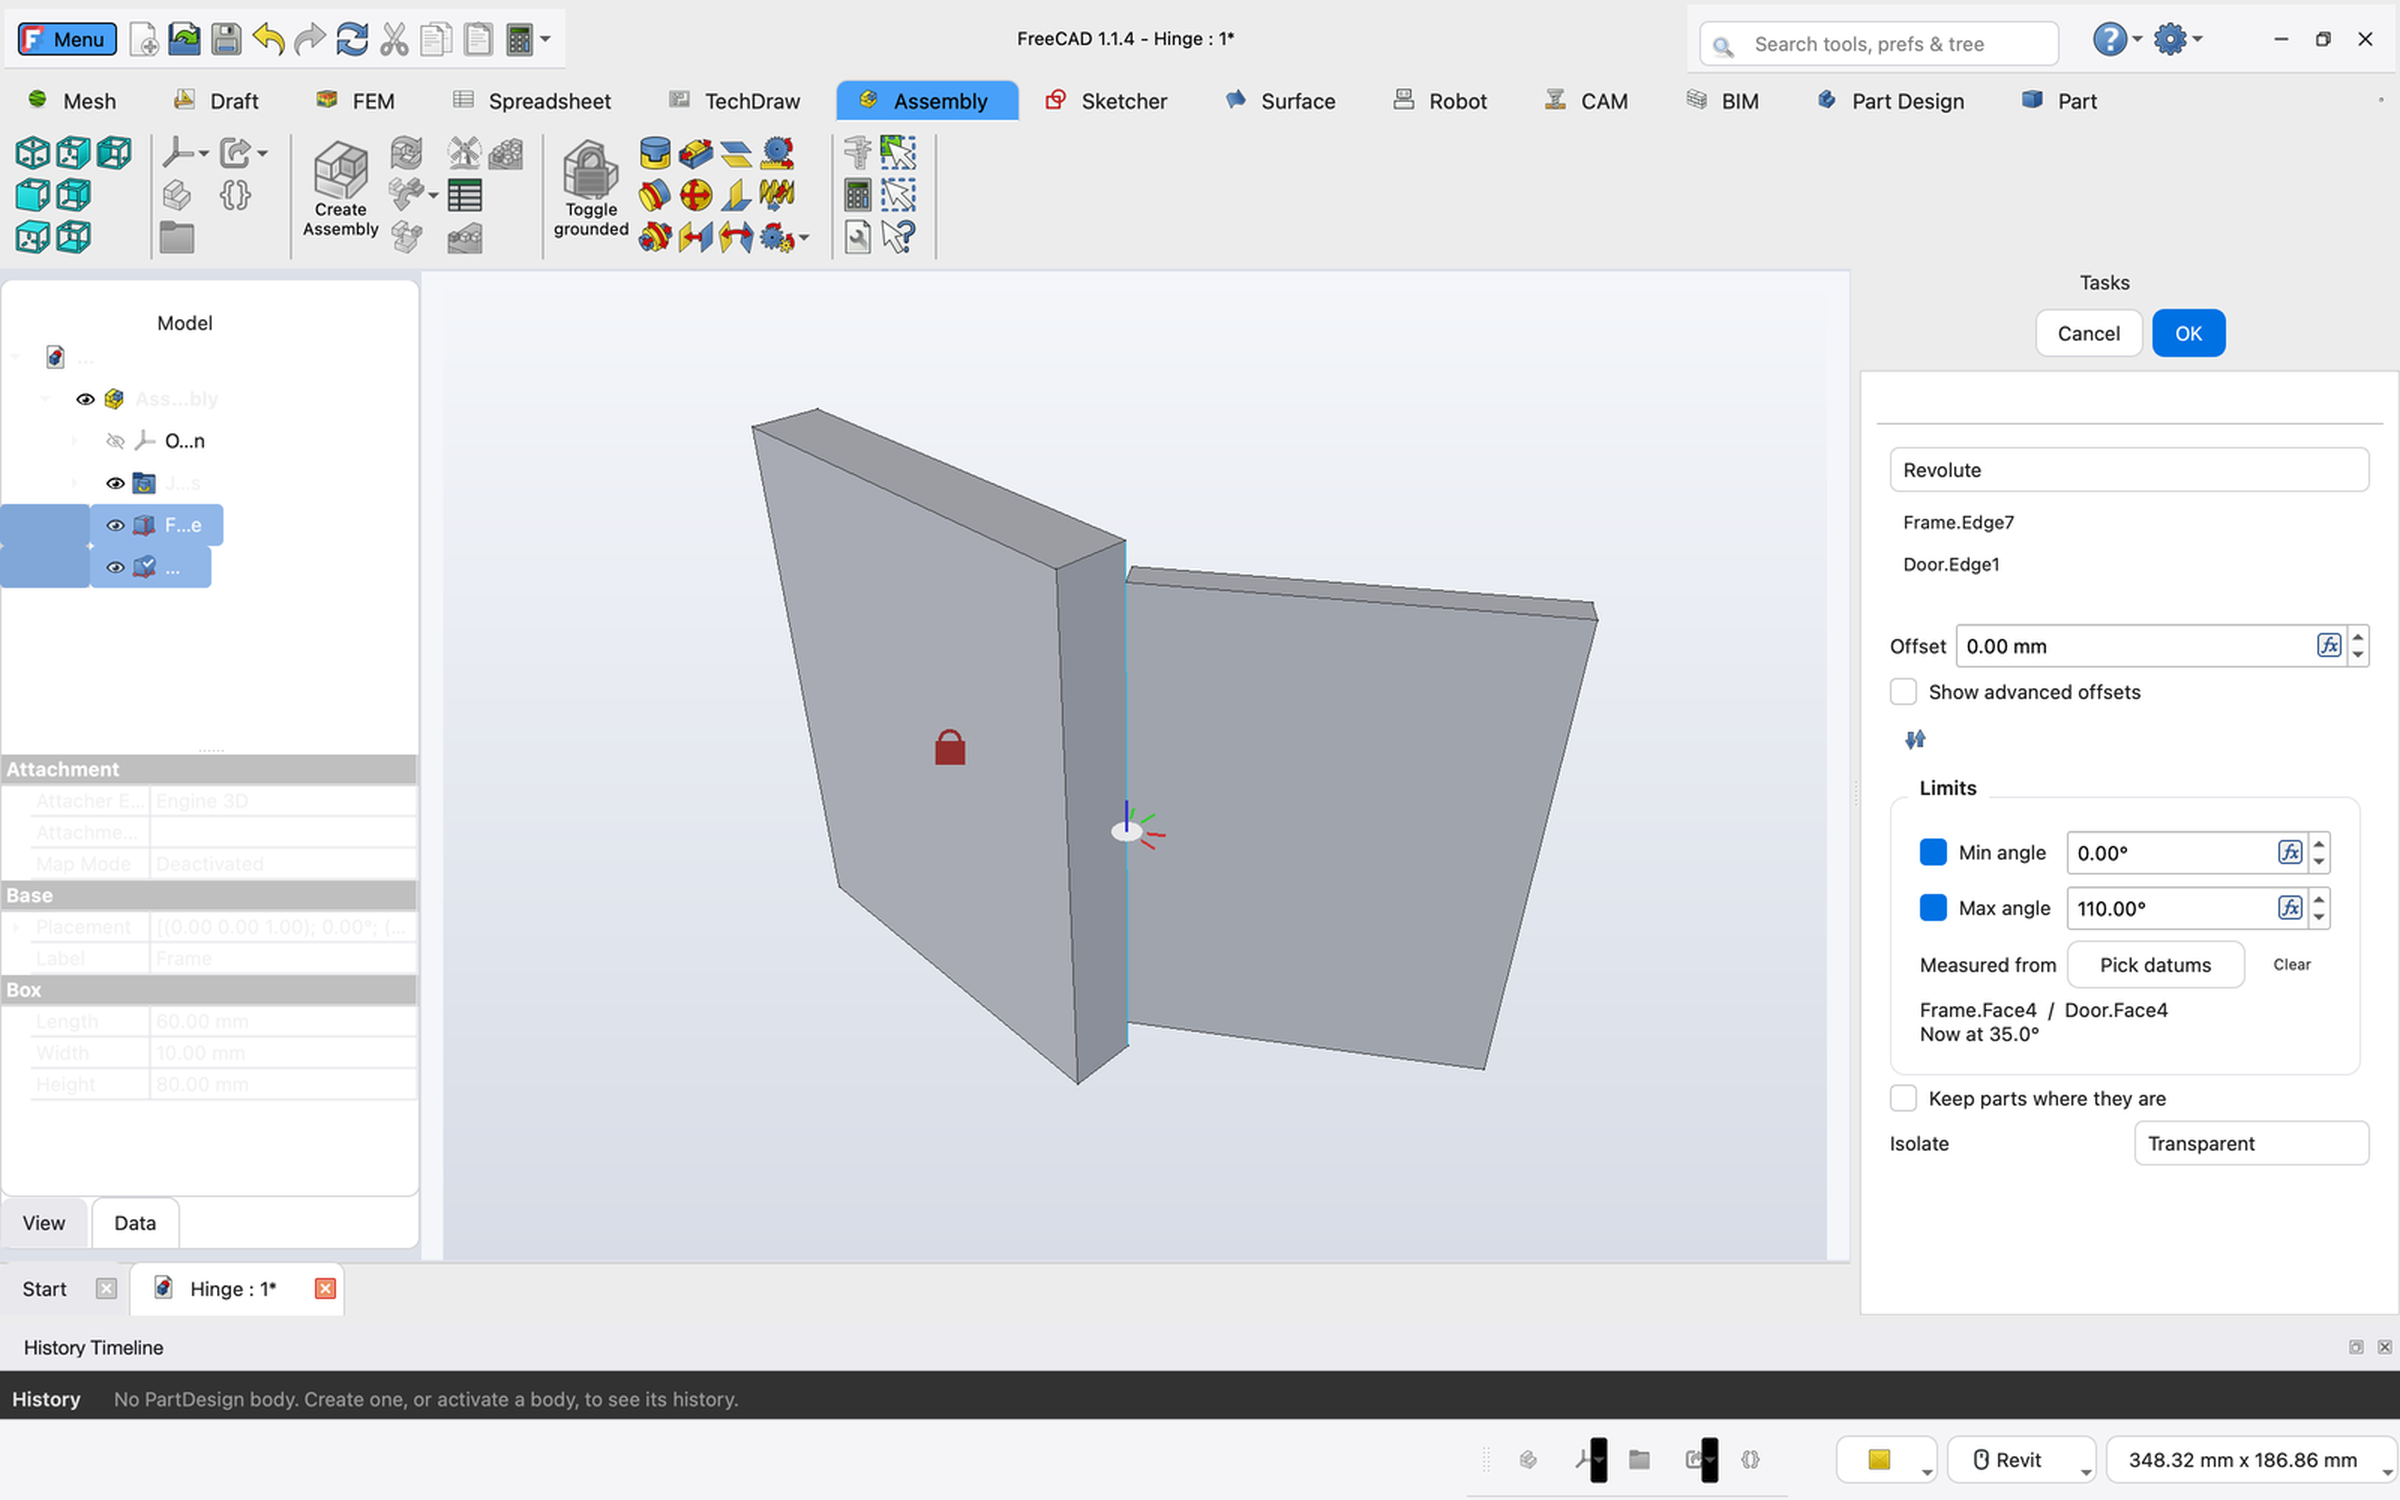
\includegraphics[width=\linewidth]{fig/ui_before_joint.png}};
  \begin{scope}[x={(img.south east)},y={(img.north west)}]
    \foreach \n/\x/\y in {1/0.035/0.972, 2/0.435/0.972, 3/0.985/0.977, 4/0.10/0.78, 5/0.175/0.53, 6/0.78/0.79, 7/0.80/0.49, 8/0.12/0.145, 9/0.05/0.105, 10/0.61/0.026}
      \node[circle,fill=bwred,text=white,font=\scriptsize\bfseries,inner sep=1.2pt,minimum size=13pt,draw=white,line width=0.8pt] at (\x,\y) {\n};
  \end{scope}
\end{tikzpicture}
\caption{This build tonight (the hinge from tests 14 and 16), with the problems numbered.}
\label{fig:ui-before}
\end{figure}

\begin{center}
\small
\begin{tabularx}{\linewidth}{@{}cXX@{}}
\toprule
\# & What you see & Cause and fix\\
\midrule
\marker{1} & ``Menu'' button, 13 workbench tabs, a large icon grid & The \textbf{FreeCAD-Ribbon} add-on (v1.12.0dev) in your FreeCAD profile, not BruceWorx. It is replaced by the BruceWorx bar; see question~3.\\
\marker{2} & Title shows ``FreeCAD 1.1.4 -- Hinge : 1*'' & Window title: the document name only, with the unsaved mark on its tab.\\
\marker{3} & Windows-style $-\,\square\,\times$ at the top right & Probably drawn by Ribbon. \verify{} Native macOS buttons (\eref{UIX-02}) come back once it is off.\\
\marker{4} & Model tree names cut short and faded (``Ass\ldots bly'', ``F\ldots e'') & The faded names have about 1.1:1 contrast. Suspected: the floating-tree sheet's white text (\file{BruceWorxModelTree.qss}) applied to a light panel, and a narrow first column. \verify\\
\marker{5} & Property headers grey on grey & Header colour from the Ribbon sheet; replaced by the token colours below.\\
\marker{6} & ``Tasks'' column the full window height, header floating & Task panel docked right. It becomes a floating command dialog with OK/Cancel at the bottom.\\
\marker{7} & Odd gaps, a stray icon, one \emph{Clear} button styled differently & Task panel layout and QSS (\eref{UIX-07}).\\
\marker{8} & Document tabs at the bottom, with red $\times$ & \code{setTabPosition(South)} is hard-coded at \file{MainWindow.cpp:397}; the red $\times$ is a stylesheet icon. \verify\\
\marker{9} & Timeline with two headers that says ``No PartDesign body'' in an assembly & Dock title plus bar header. It becomes one row and is hidden when there is no history.\\
\marker{10} & Status bar: black bars, ``Revit'', a size cut off & Status-bar widgets with no styling. \verify{} They are regrouped as quiet readouts.\\
\bottomrule
\end{tabularx}
\end{center}

\subsubsection*{The design, one screen explained}

\begin{figure}[!htbp]
\centering
\begin{tikzpicture}
  \node[anchor=south west,inner sep=0] (img) at (0,0) {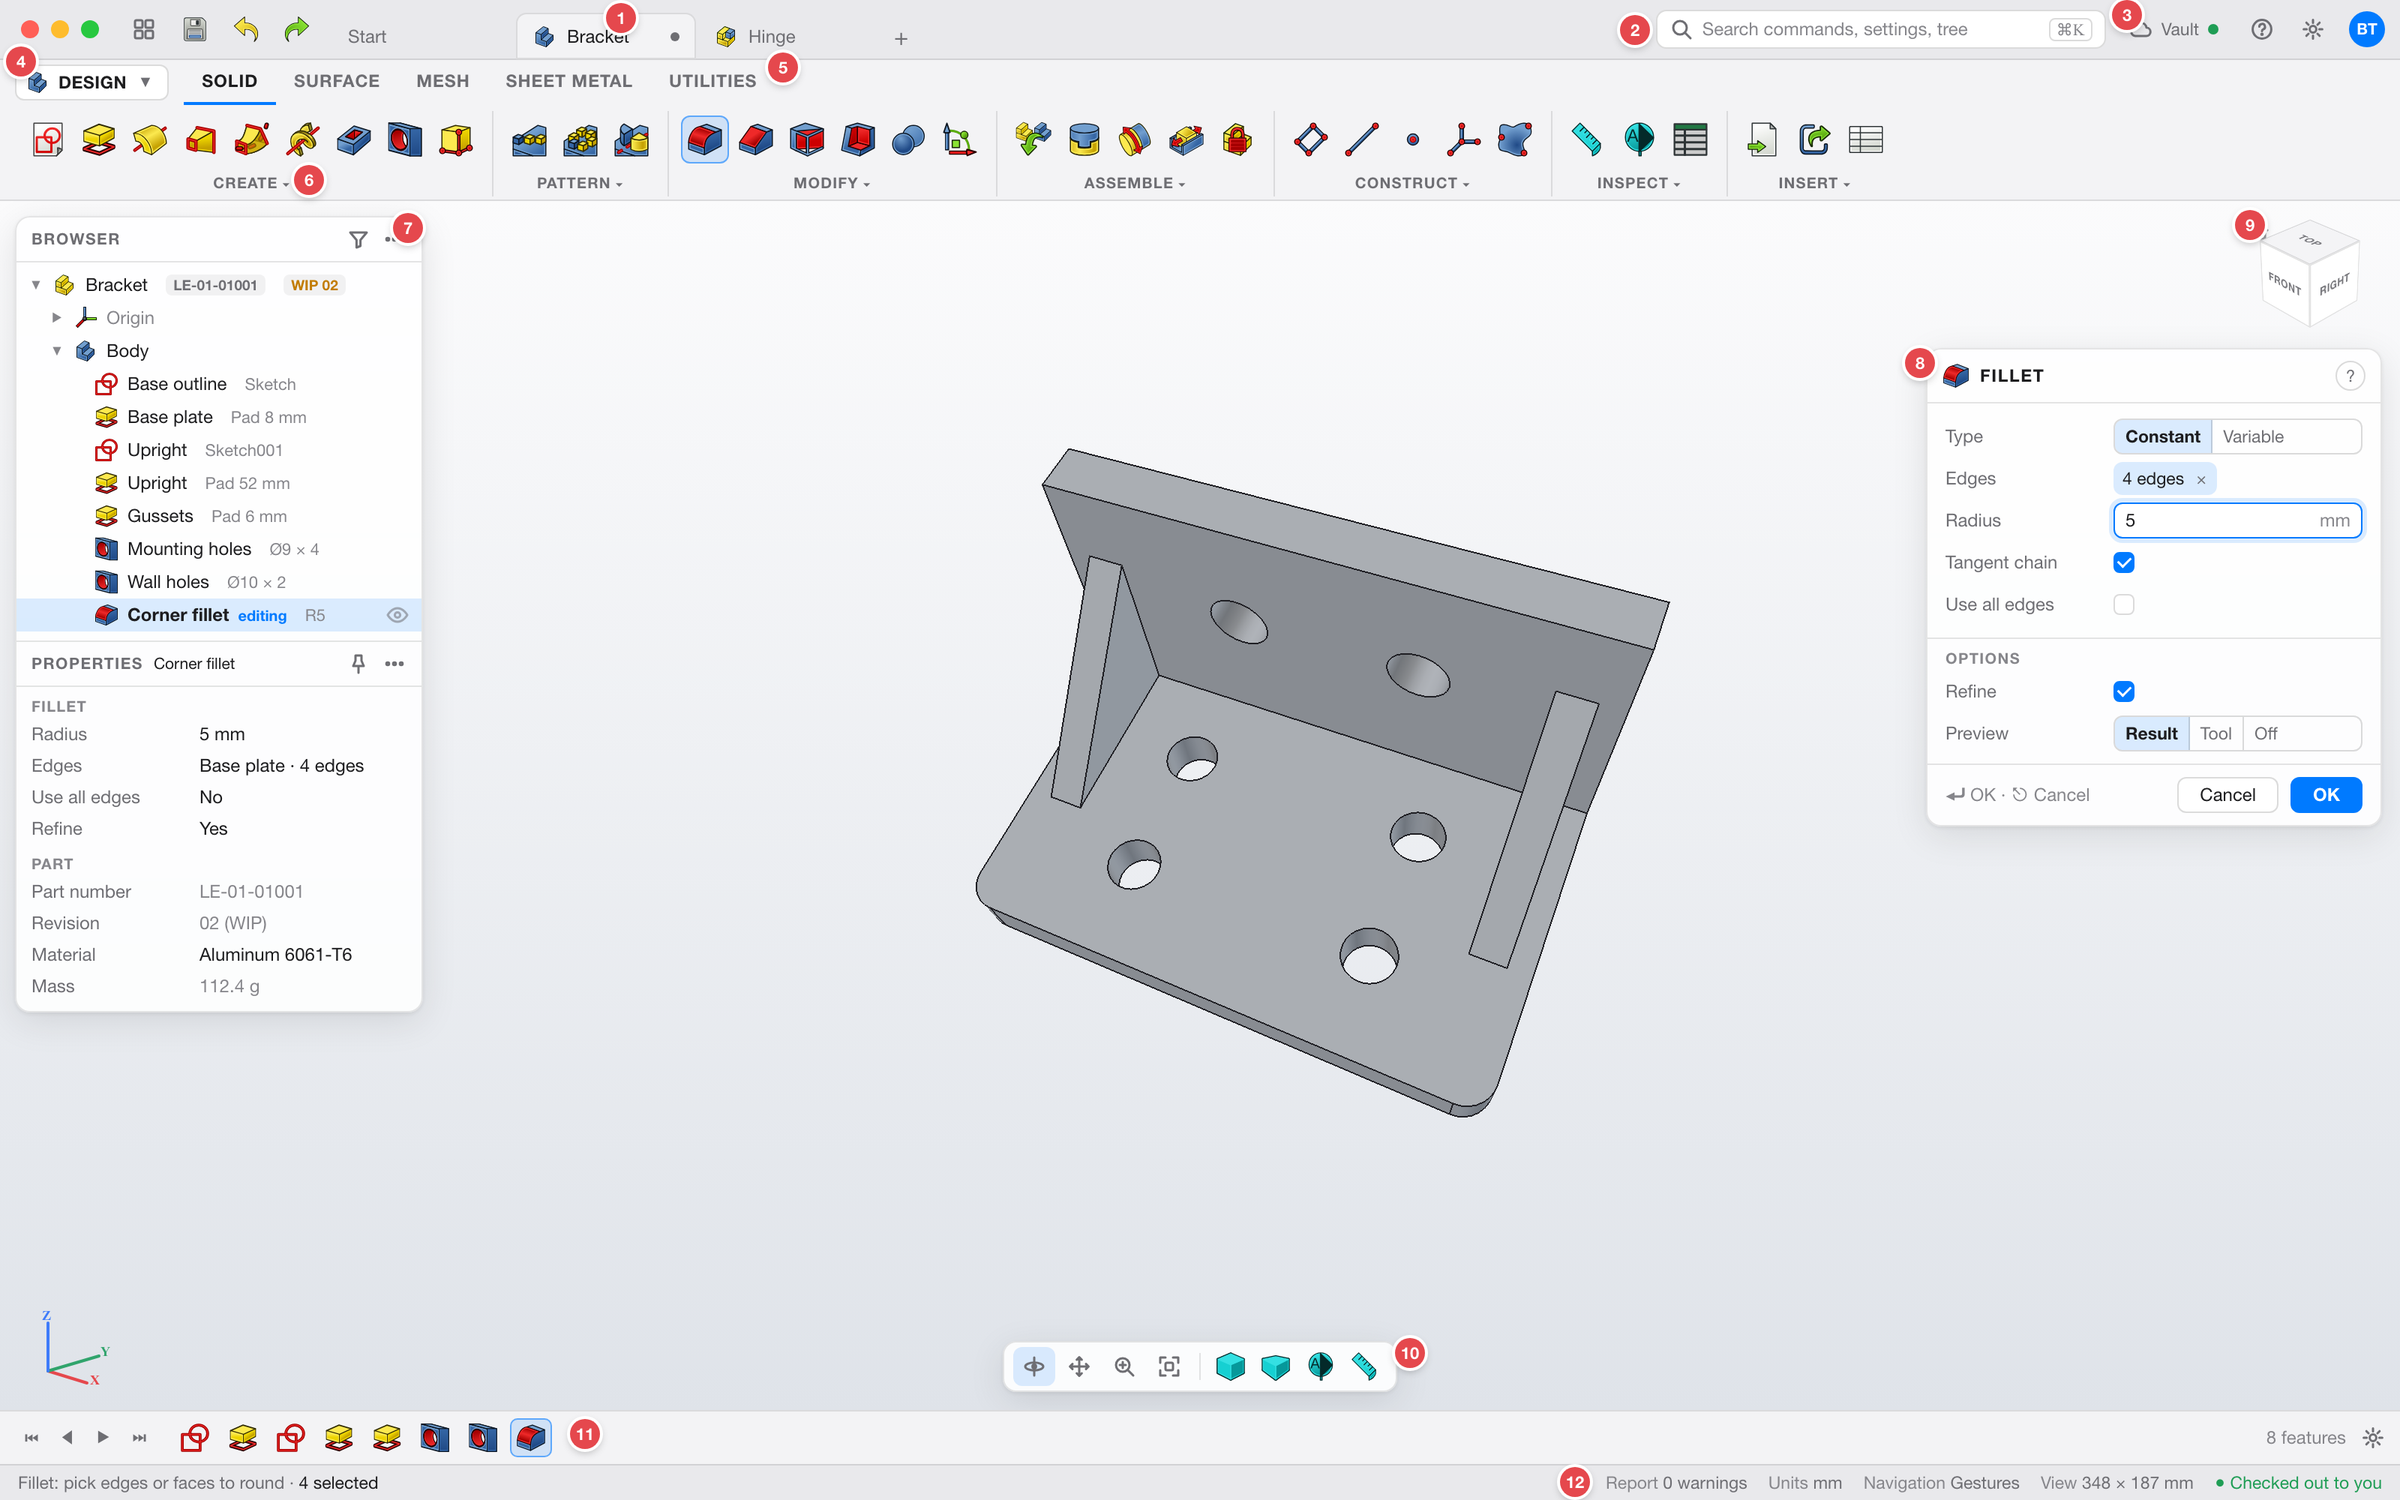
\includegraphics[width=\linewidth]{fig/ui_mock_part-notes.png}};
\end{tikzpicture}
\caption{Part modelling, light. A body with a fillet being edited. The numbers match the table below.}
\label{fig:ui-notes}
\end{figure}

\begin{center}
\small
\begin{tabularx}{\linewidth}{@{}cp{3.3cm}Xl@{}}
\toprule
\# & Element & How it is built & Epic\\
\midrule
\marker{1} & Document tabs in the title bar & Tab bar moved \code{North} (a preference instead of the hard-coded \code{South}), then hosted in the unified title bar. Modified dot instead of $\times$; $\times$ on hover. & \eref{UIX-06}\\
\marker{2} & Search, \texttt{Cmd-K} & Commands, preferences and tree in one field. Built in, or the SearchBar add-on restyled (question~2). & \eref{UIX-06}\\
\marker{3} & Vault status & Small Python status widget reading the folder vault (\S\ref{sec:pdm-eval}). & \eref{PDM-04}\\
\marker{4} & Workspace menu & \code{WorkspaceSelector}, as in the starting brief. & \eref{UIX-05}\\
\marker{5} & Tabs, plus \textsc{Sketch} in accent while a sketch is open & Toolbar sets per tab; the contextual tab is pushed on sketch edit. & \eref{UIX-05}\\
\marker{6} & Captioned groups, 24\,px icons & One icon size (preference), each toolbar given a caption and a $\blacktriangledown$ overflow menu. No icon is redrawn. & \eref{UIX-06}\\
\marker{7} & Browser with properties & Tree and property view in the left overlay as one card. Second column shows the feature summary (``Pad 8 mm''), P/N and state badges from the part properties (\S\ref{sec:partprops}). & \eref{UIX-03}\\
\marker{8} & Command dialog & Task panel in the right overlay as a card. Icon and title header, OK/Cancel at the bottom (\code{TaskDialog::South} as default), keyboard hint. & \eref{UIX-07}\\
\marker{9} & View cube & NaviCube size, colours and font are already preferences. & \eref{UIX-01}\\
\marker{10} & Navigation pill & Small Python overlay on the 3D view: orbit, pan, zoom, fit, display style, camera, section, measure. & \eref{UIX-06}\\
\marker{11} & Timeline, one row & HistoryTimeline mod: no dock title, 20\,px icons, rolled-back items dimmed. & \eref{UIX-04}\\
\marker{12} & Status bar & Prompt on the left; Report, units, navigation style, view size and vault state on the right, as text. & \eref{UIX-06}\\
\bottomrule
\end{tabularx}
\end{center}

\subsubsection*{What ``clean but feature dense'' means in numbers}

Dense means more on screen without a smaller target. Clean means one of everything: one icon size per place,
one corner radius per kind of thing, one accent. Every size is a multiple of 2\,px on a 4\,px grid.

\begin{center}
\small
\begin{tabularx}{\linewidth}{@{}lXl@{}}
\toprule
Thing & Rule & Today\\
\midrule
Text & 12\,px system font (SF Pro); captions 10\,px semibold capitals, letter-spaced & 13\,px (\file{BruceWorx.qss})\\
Tree rows & 22\,px; property rows 21\,px; dialog fields 28\,px & tree 28\,px, task list 42\,px\\
Icons & 24\,px toolbar, 20\,px timeline and navigation, 16\,px tree and tabs & toolbar about 22 and 40\,px mixed\\
Corners & 6\,px controls, 10\,px cards & mixed\\
Panels & Floating cards over the 3D view with a translucent, blurred background & docked columns\\
Colour & Neutral greys plus \emph{one} accent; state colours only for state (WIP, released, errors) & several blues\\
\bottomrule
\end{tabularx}
\end{center}

With 22\,px rows the Browser shows $\lfloor 560/22 \rfloor = 25$ rows in the height that holds 20 today. The ``today'' column is measured from figure~\ref{fig:ui-before} and the stylesheet. The
command dialog fits the whole Revolute joint, limits included, without scrolling.

\subsubsection*{Light and dark, following macOS}

\begin{figure}[!htbp]
\centering
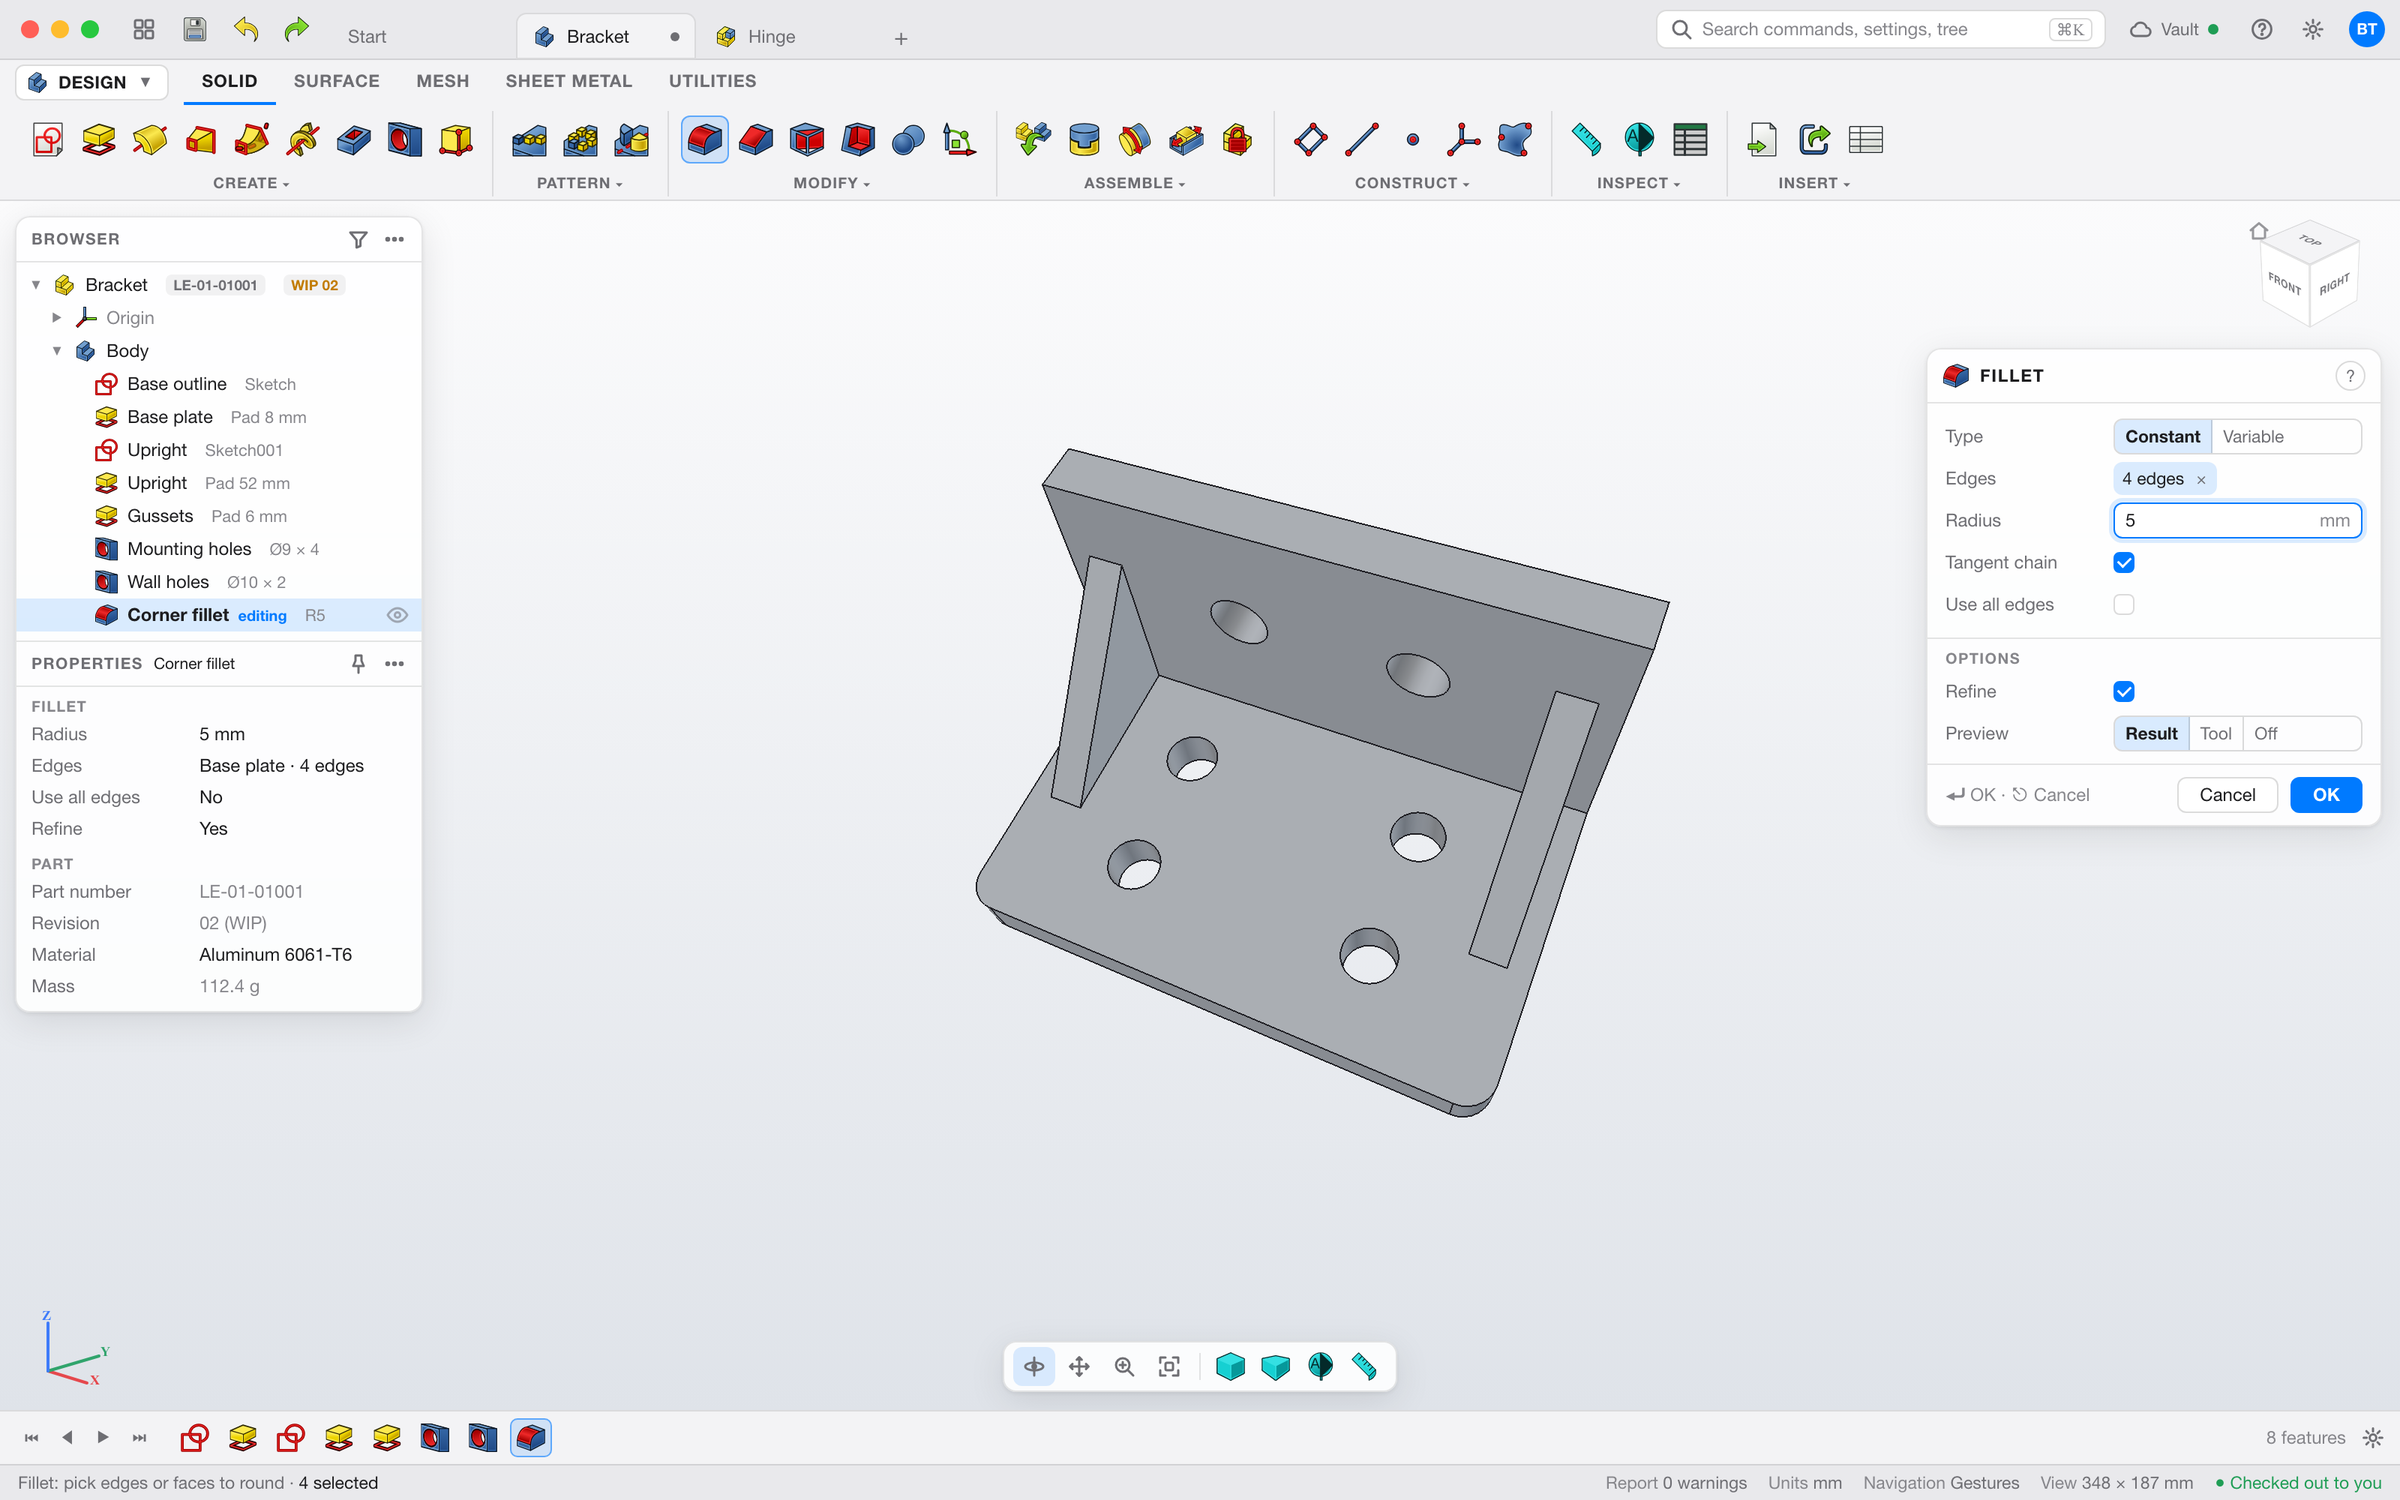
\includegraphics[width=0.497\linewidth]{fig/ui_mock_part-light.png}\hfill
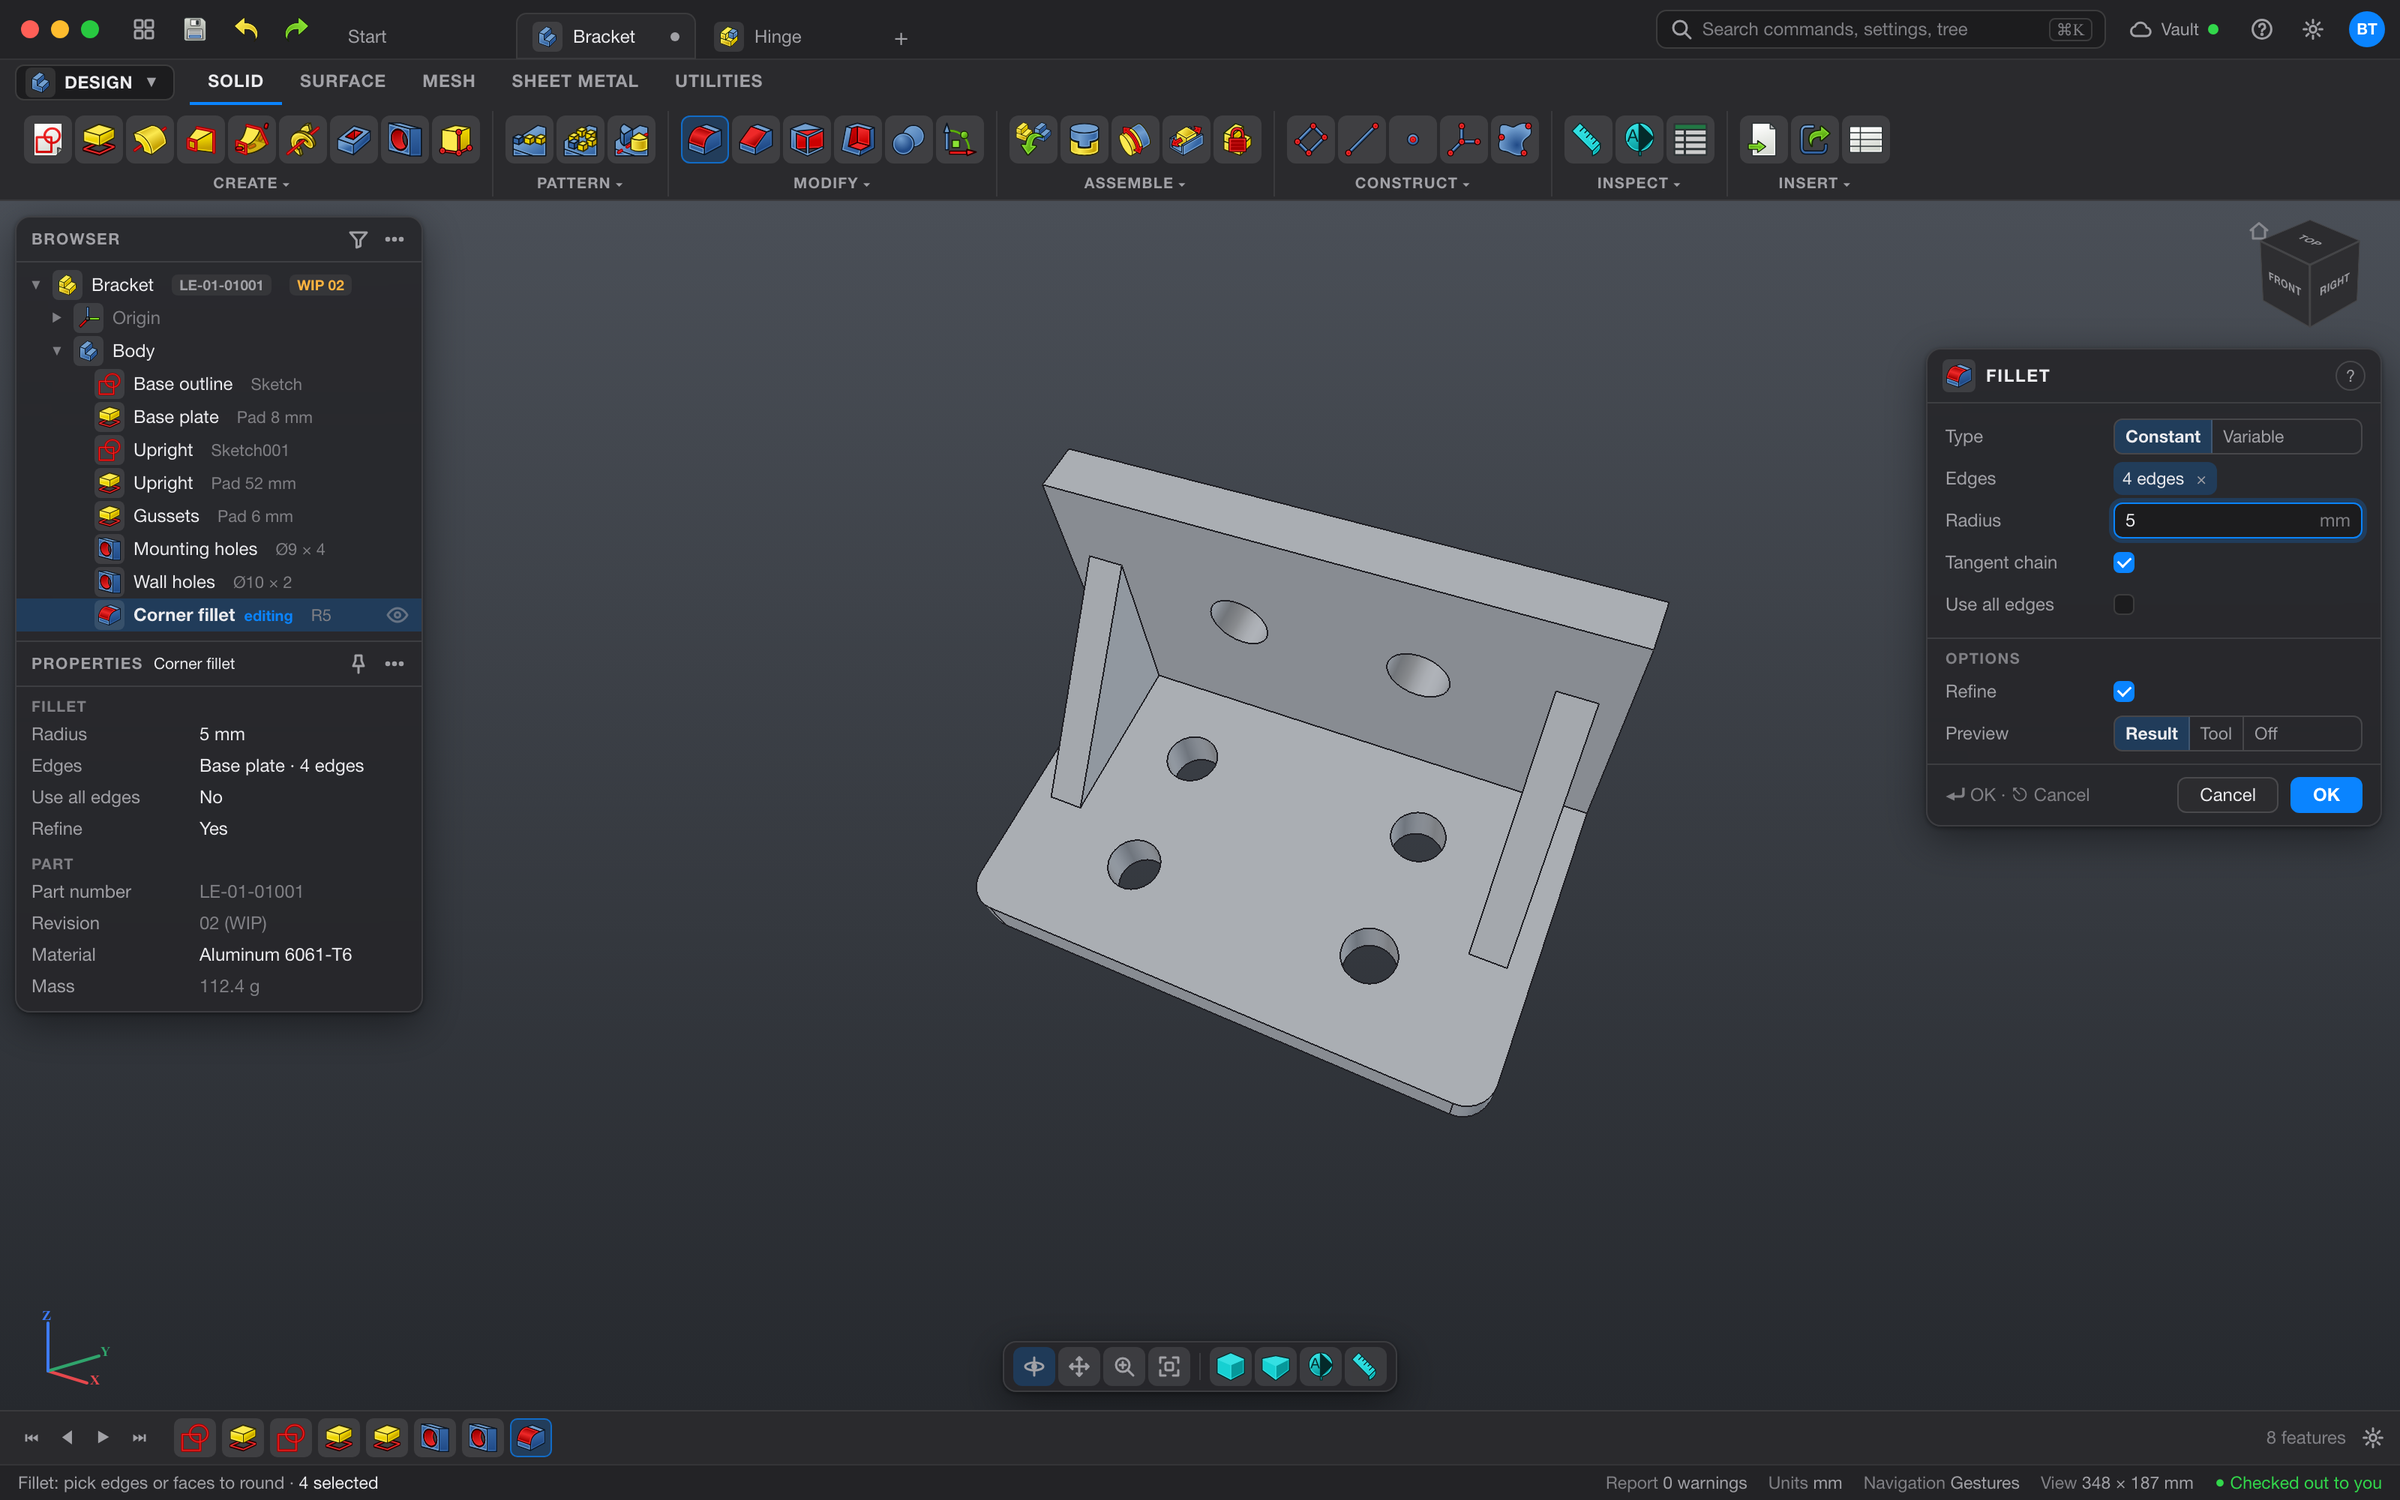
\includegraphics[width=0.497\linewidth]{fig/ui_mock_part-dark.png}\\[3pt]
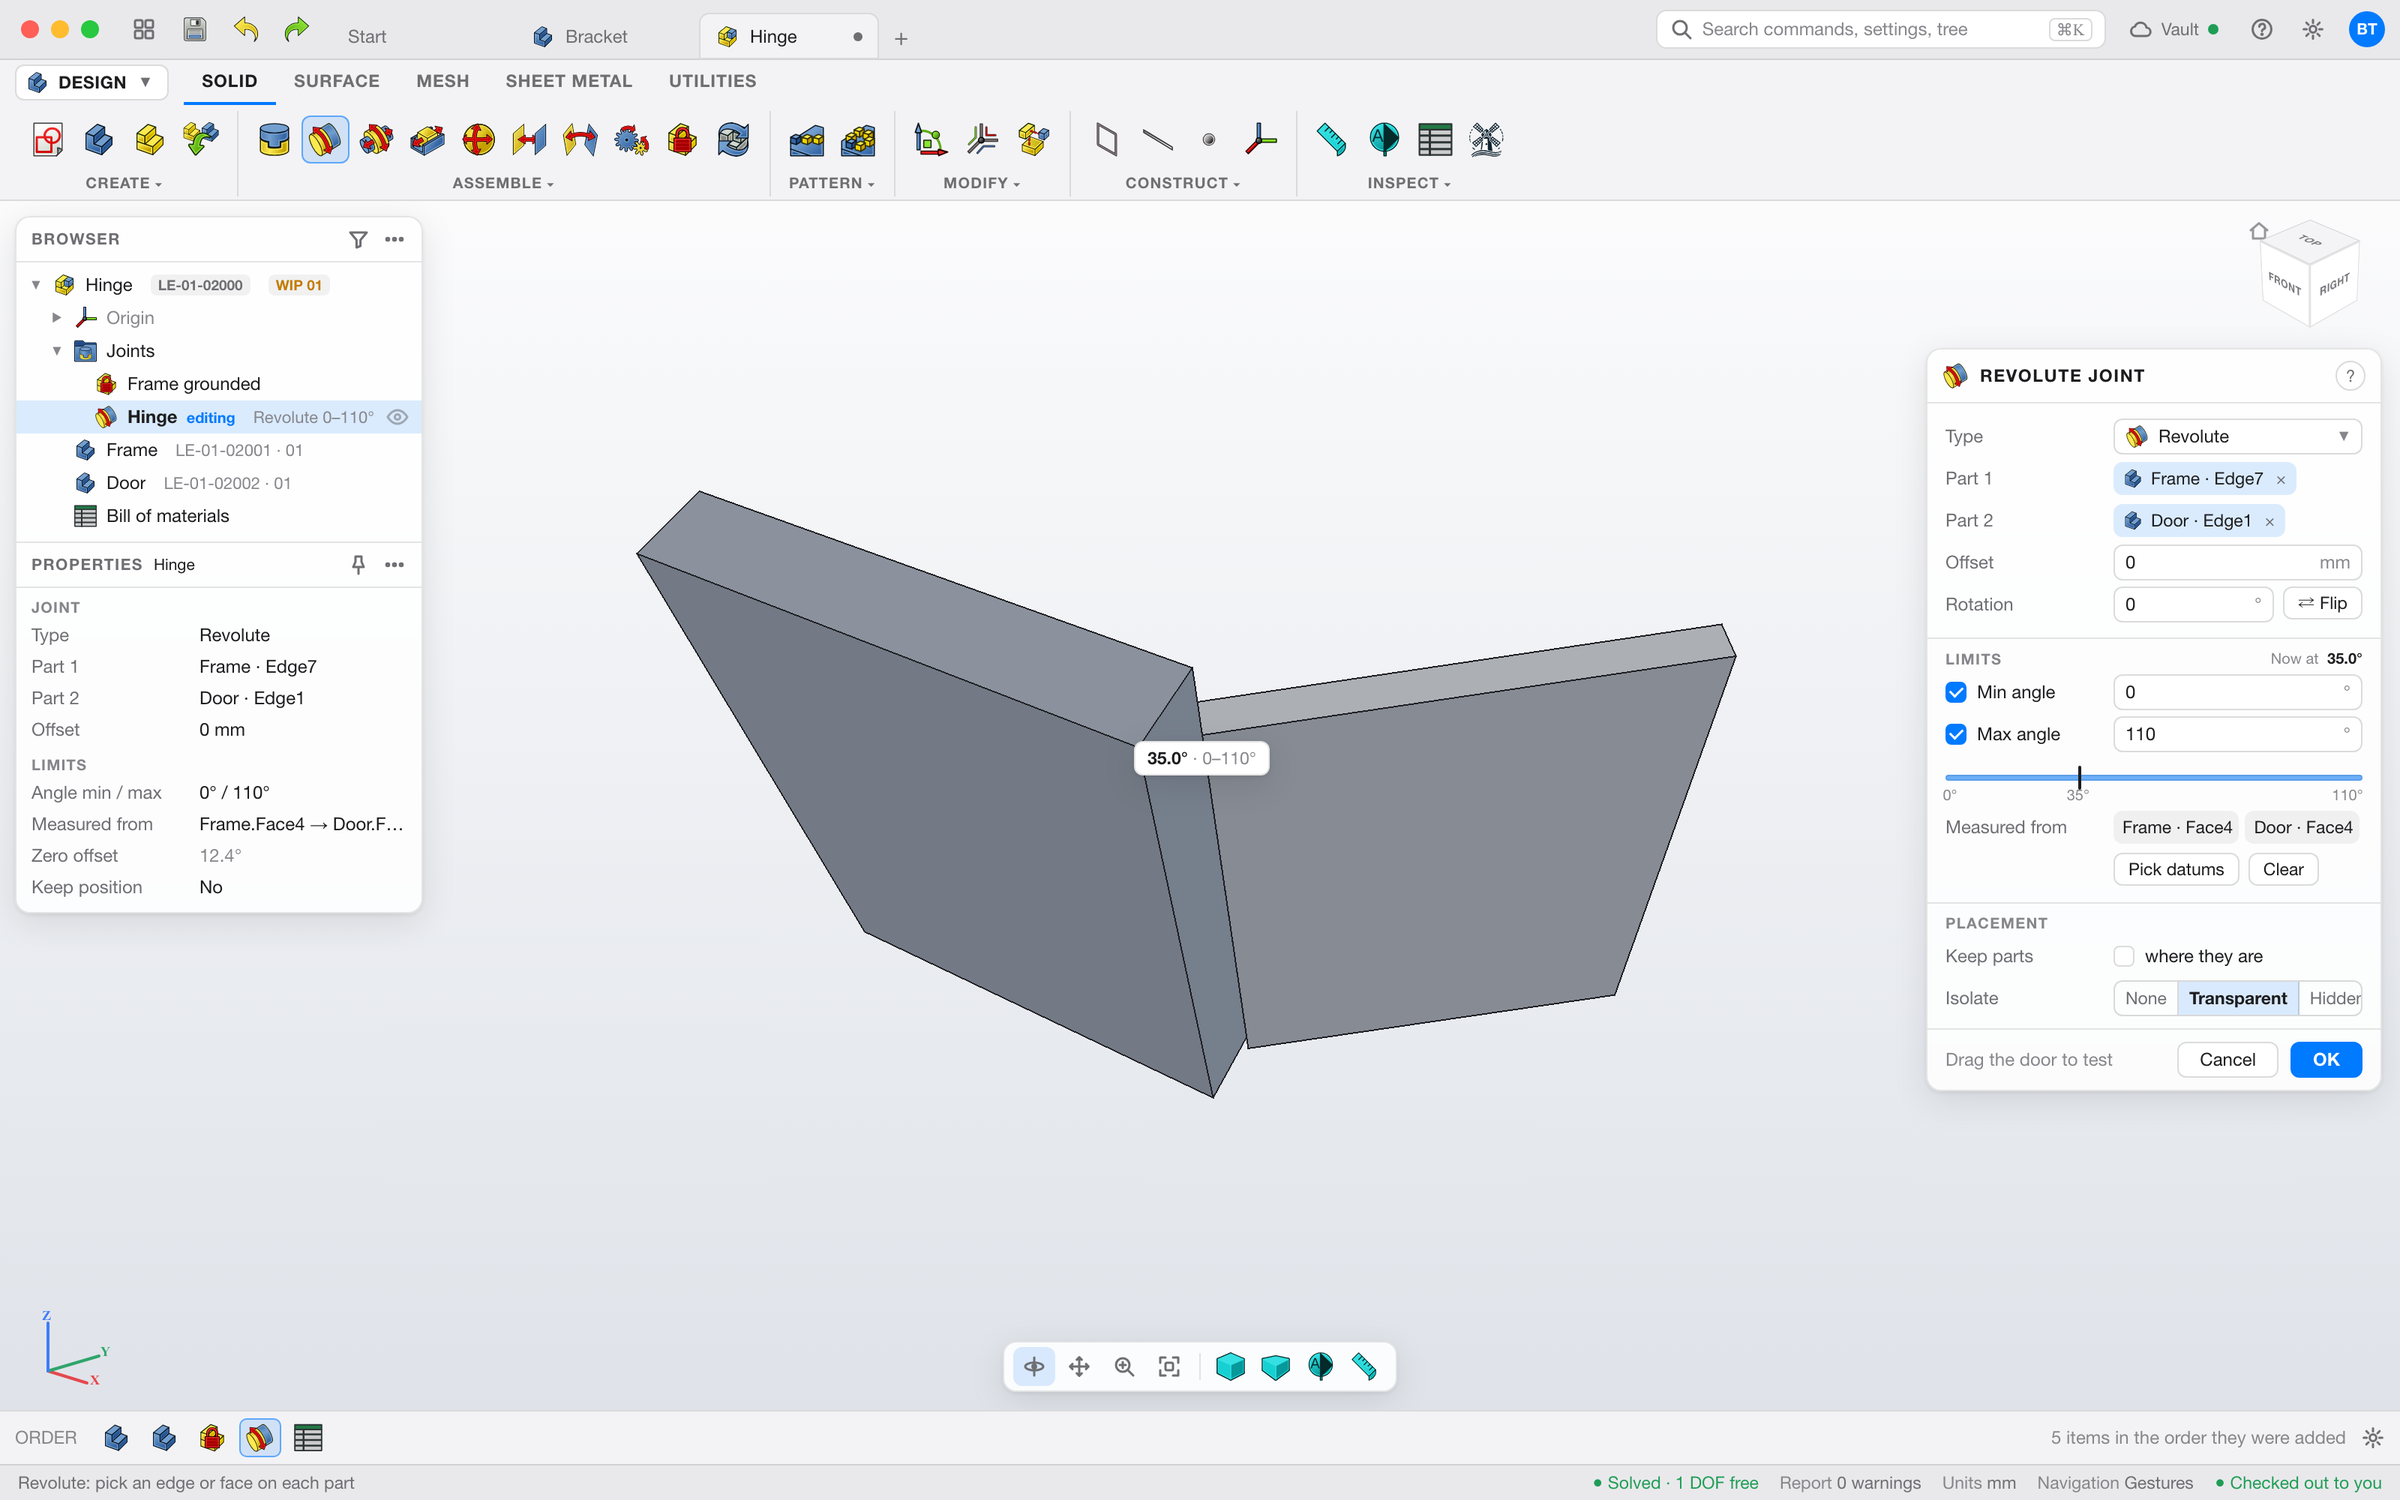
\includegraphics[width=0.497\linewidth]{fig/ui_mock_asm-light.png}\hfill
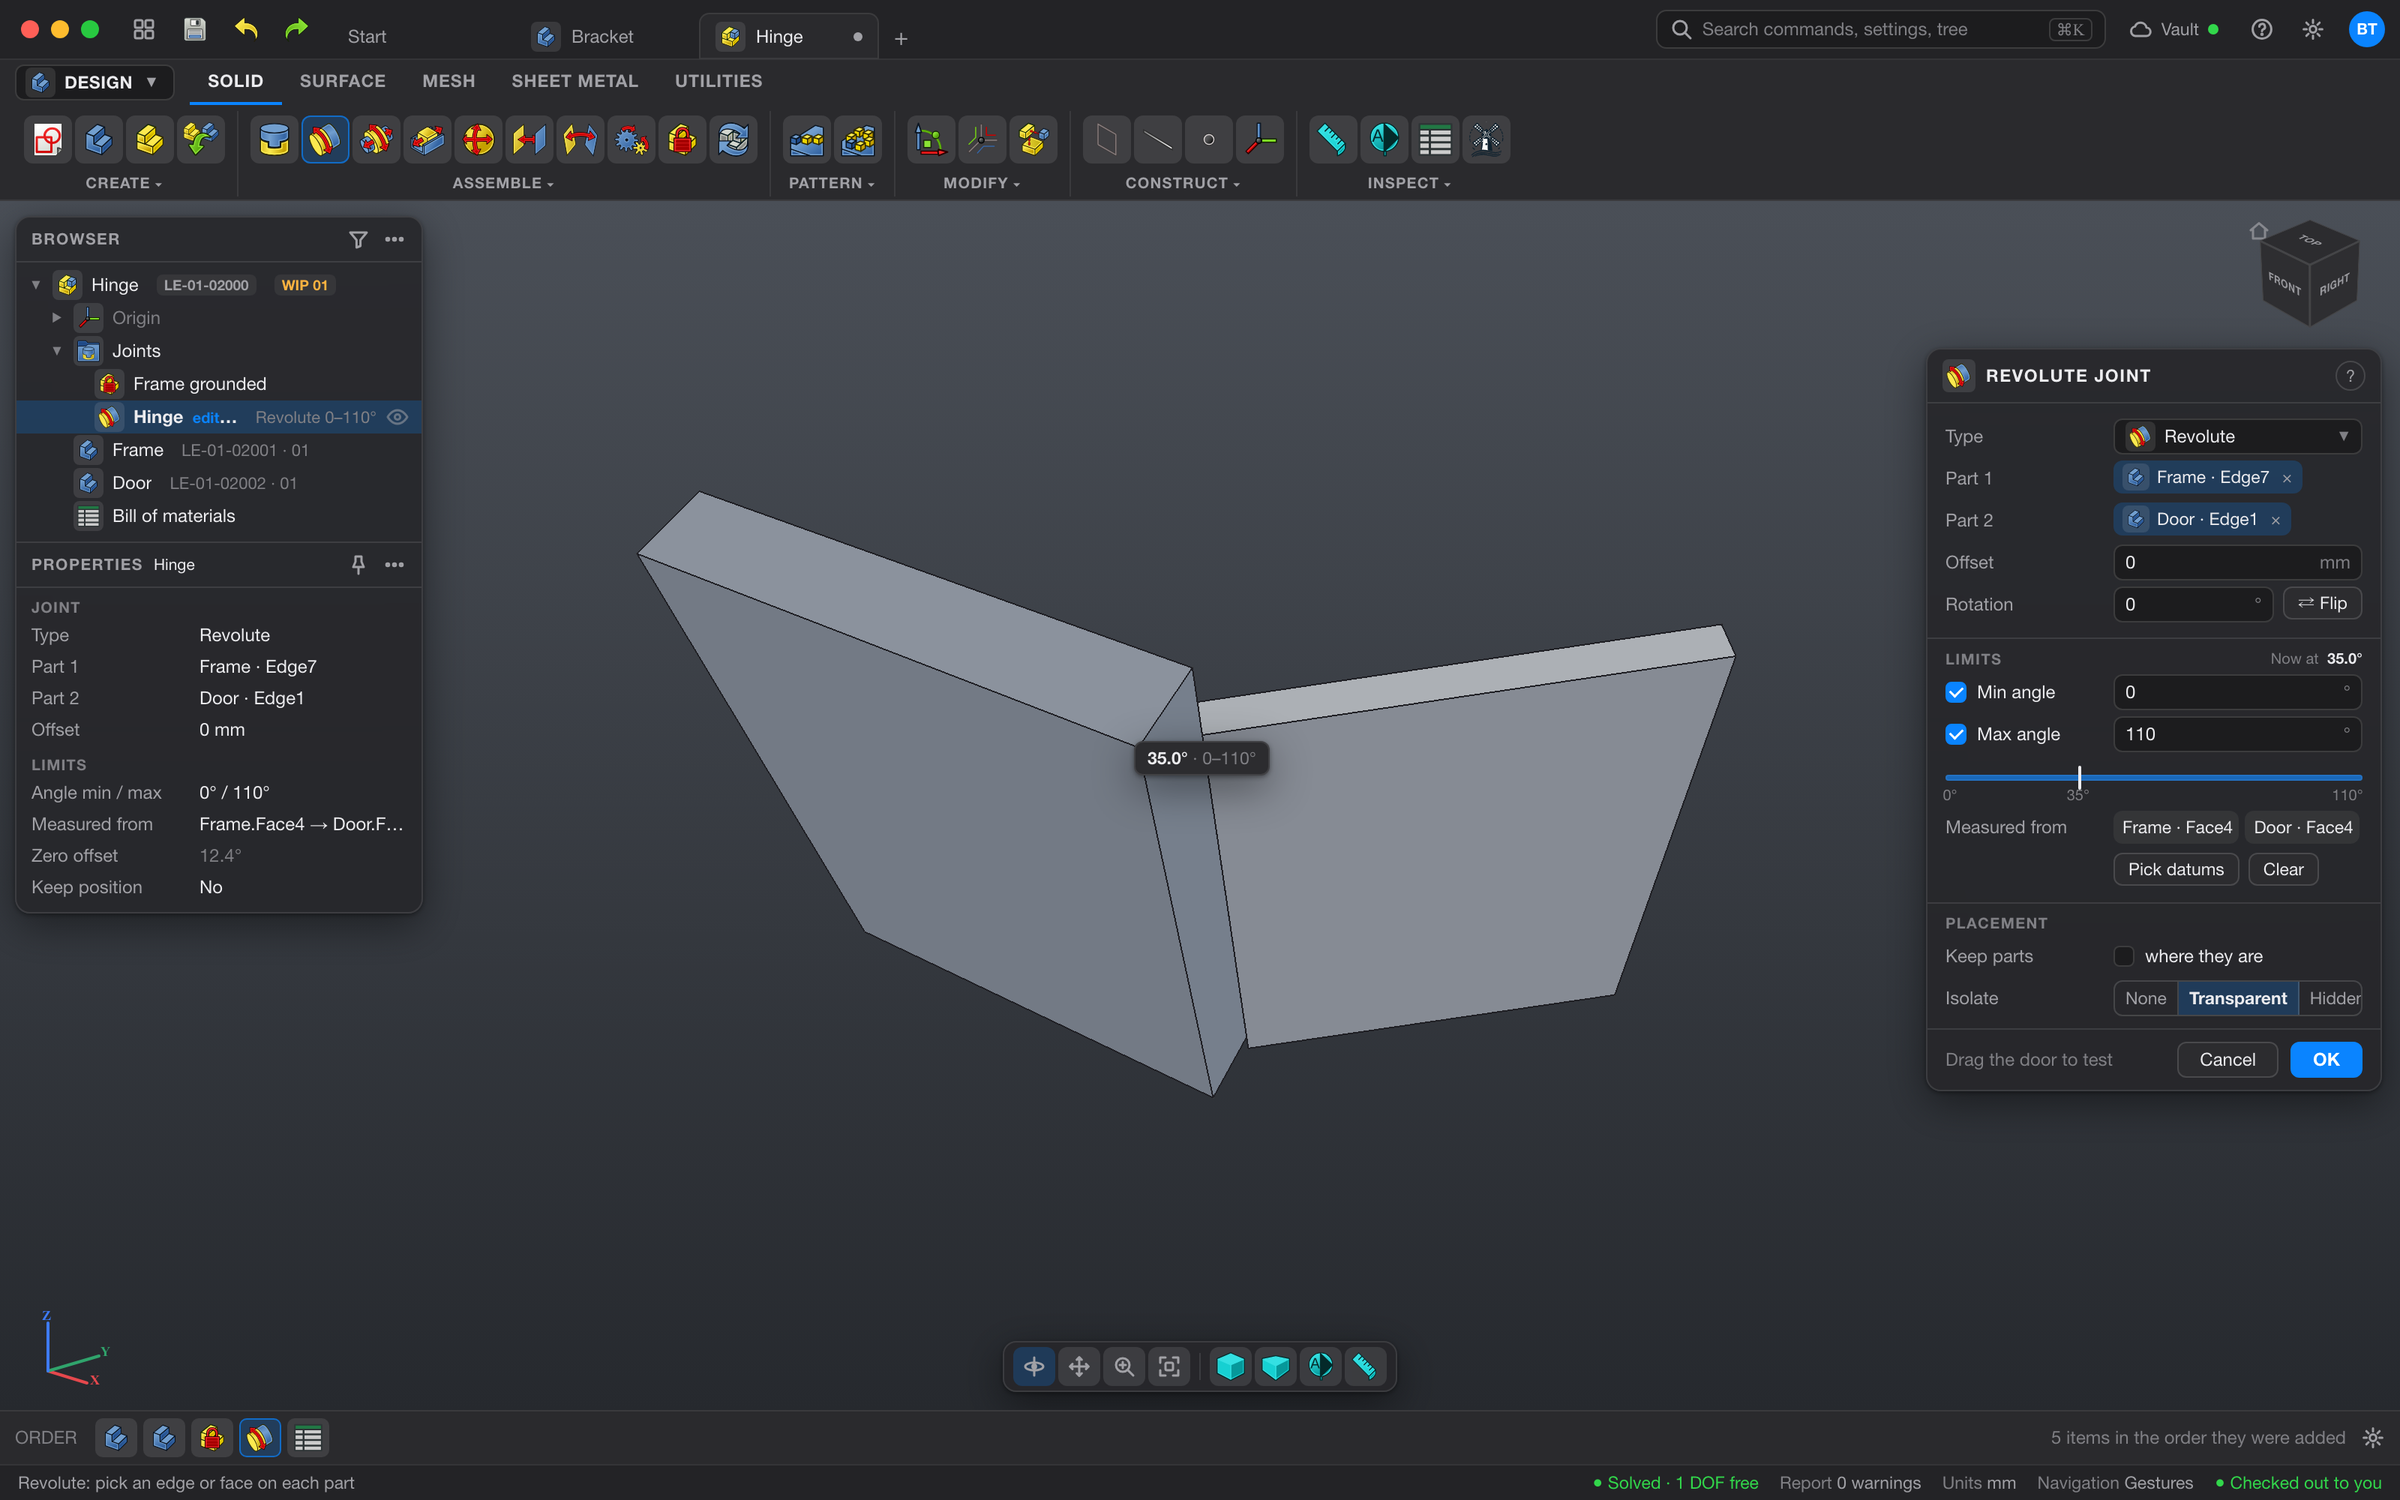
\includegraphics[width=0.497\linewidth]{fig/ui_mock_asm-dark.png}
\caption{Part modelling and assembly, light and dark. The assembly shows the Revolute joint from section
\ref{sec:joints}. The limits get a range bar with the current reading, ``Measured from'' shows both datums, and
the angle is labelled in the 3D view. Assemblies have no feature history, so the timeline row says so instead of
showing a PartDesign message.}
\label{fig:ui-part-asm}
\end{figure}

\begin{figure}[!htbp]
\centering
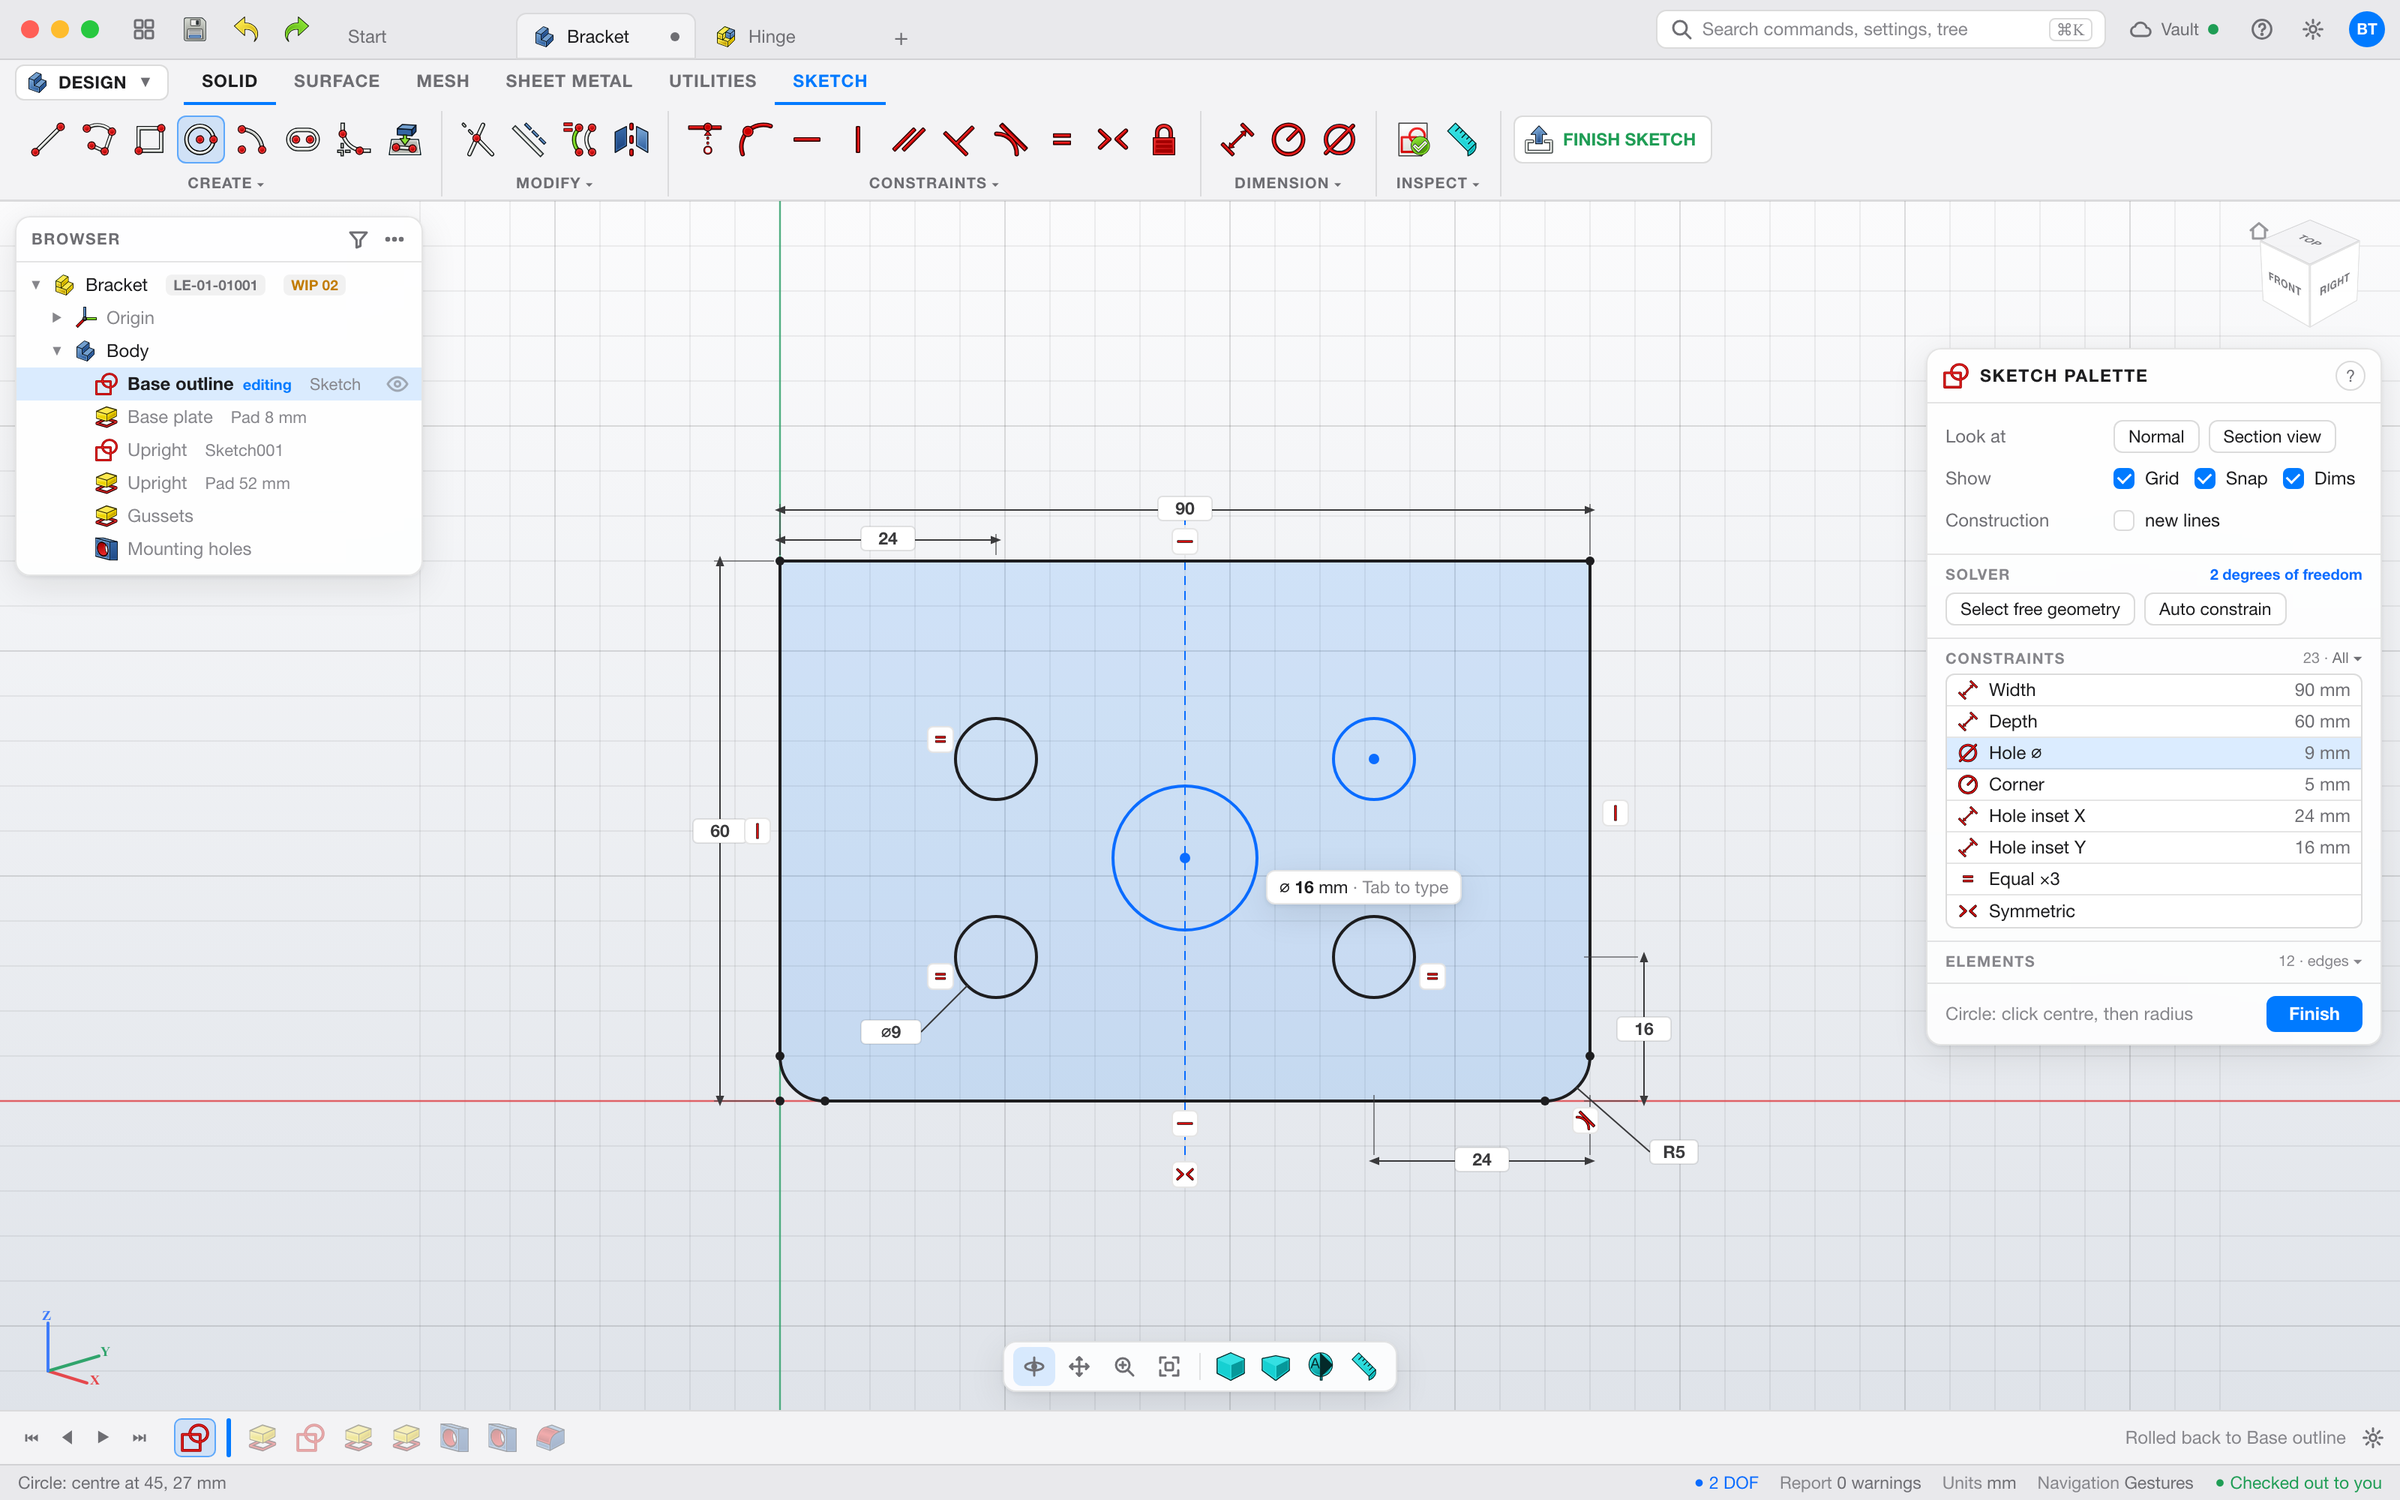
\includegraphics[width=0.497\linewidth]{fig/ui_mock_sketch-light.png}\hfill
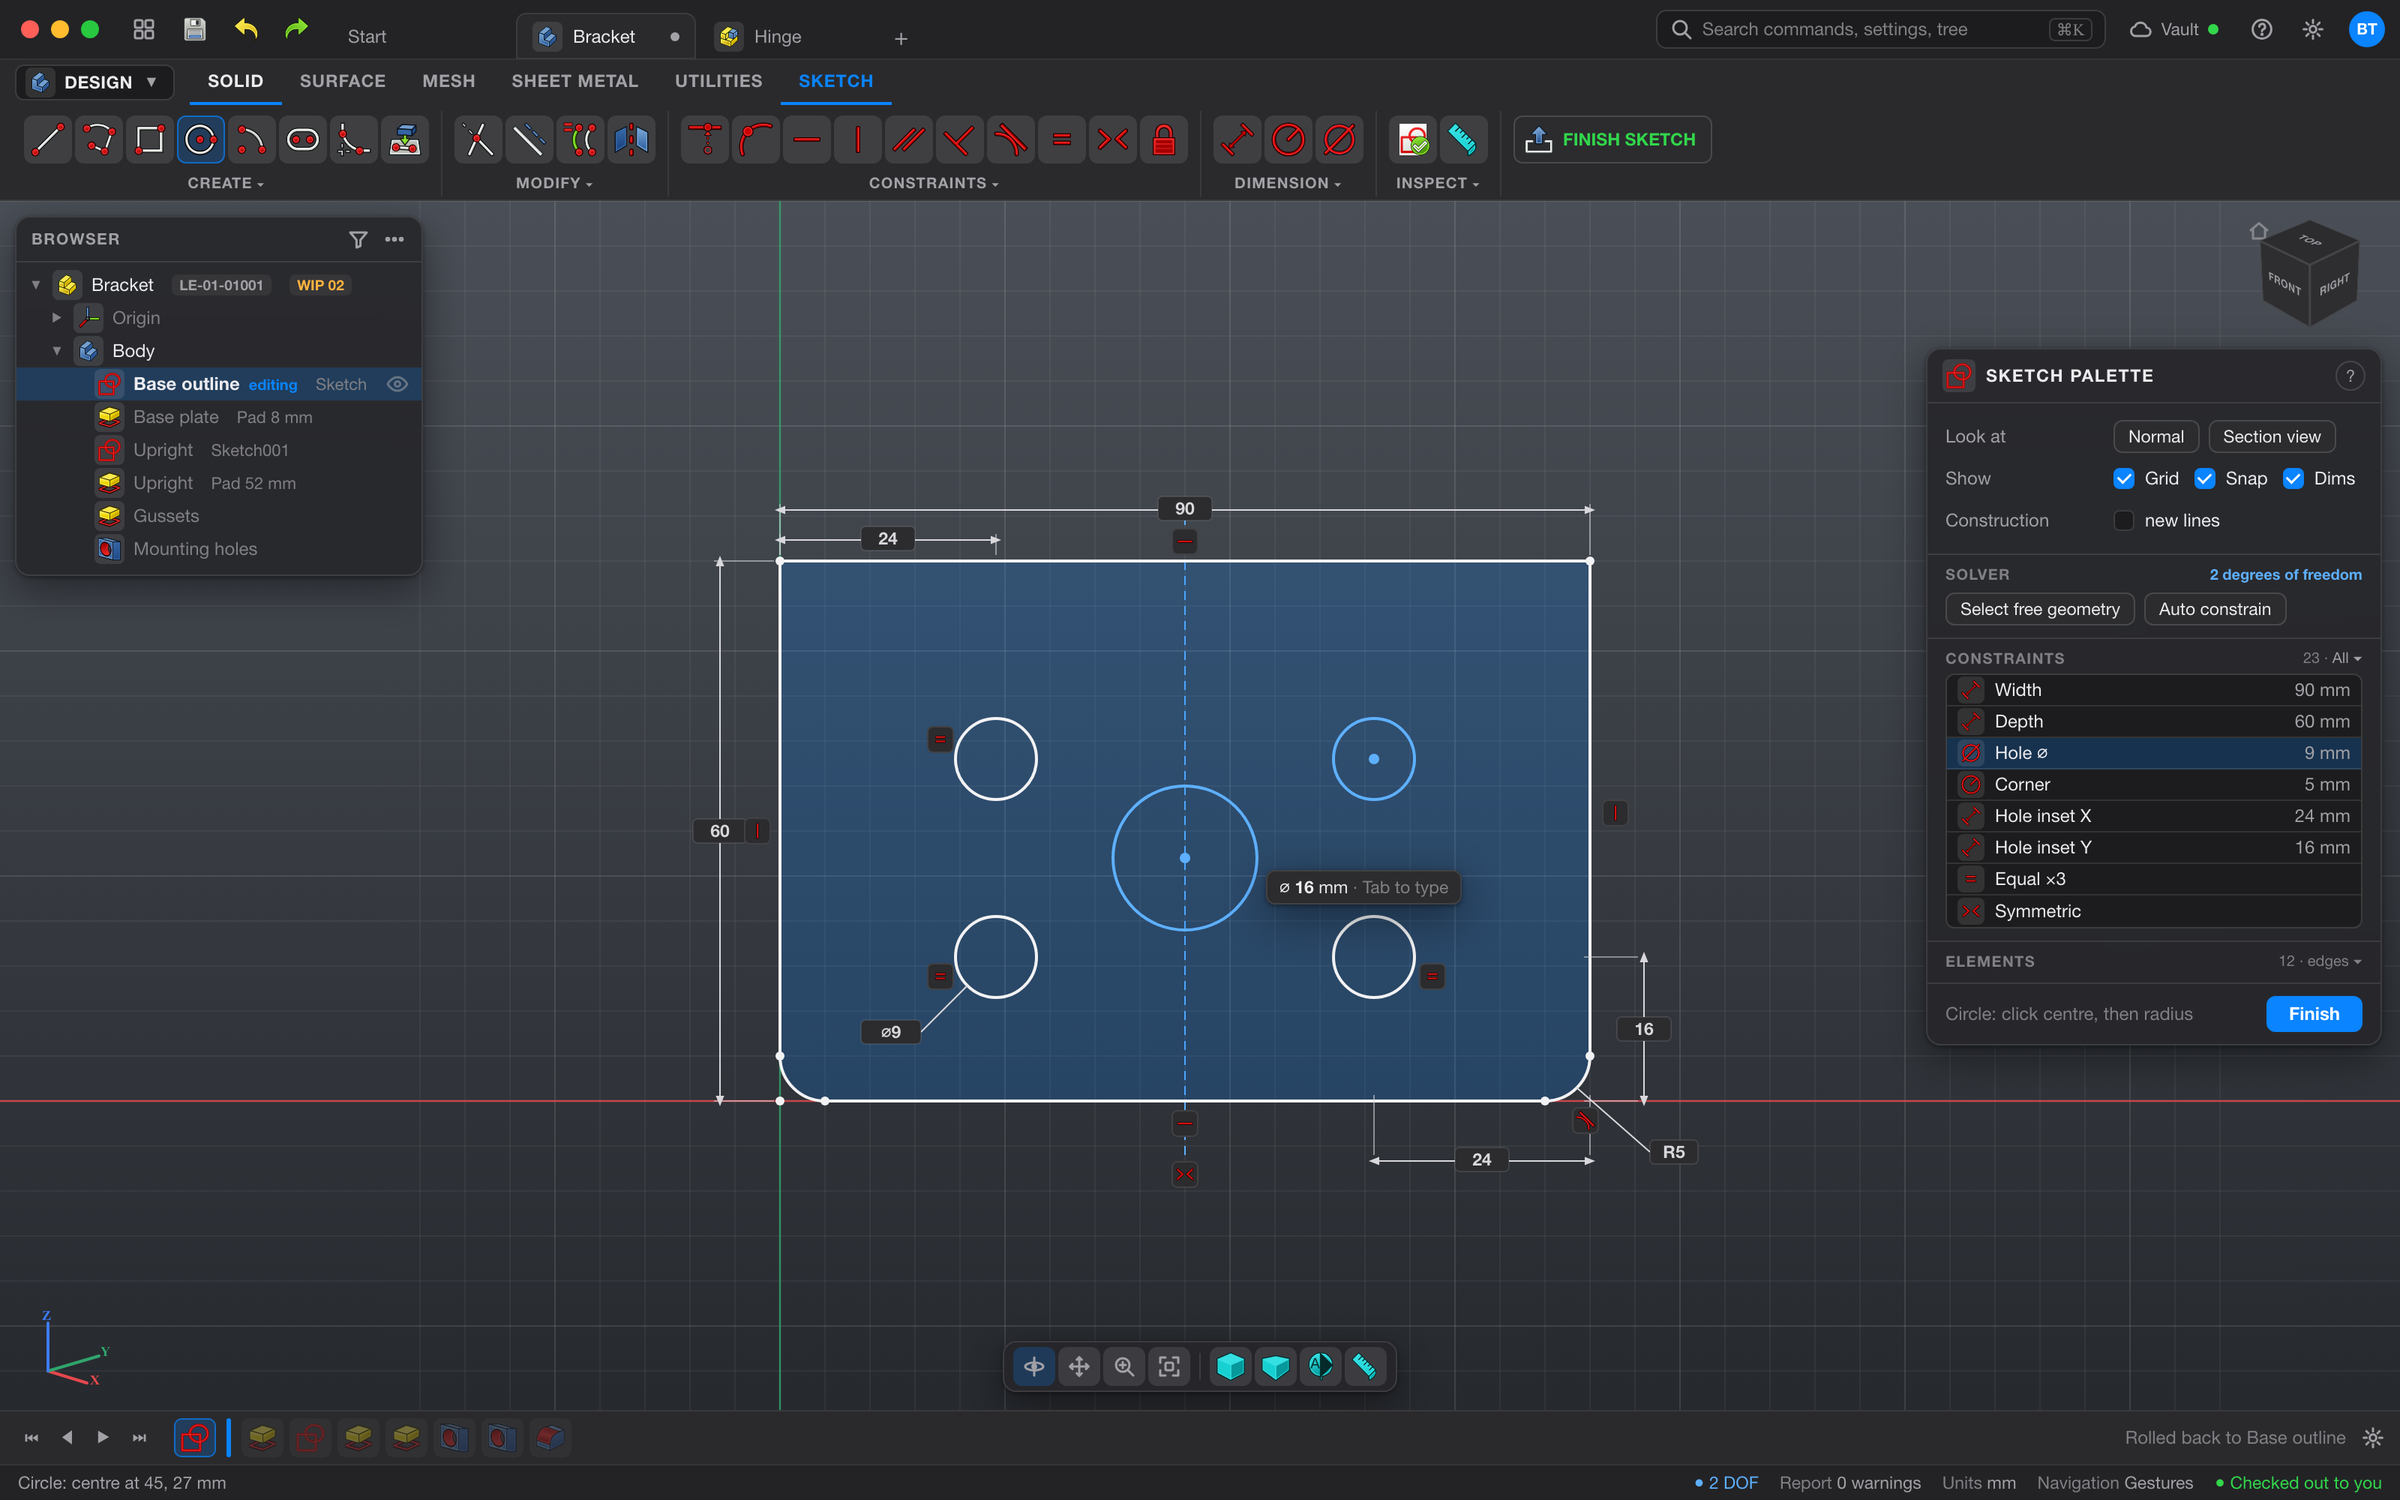
\includegraphics[width=0.497\linewidth]{fig/ui_mock_sketch-dark.png}\\[3pt]
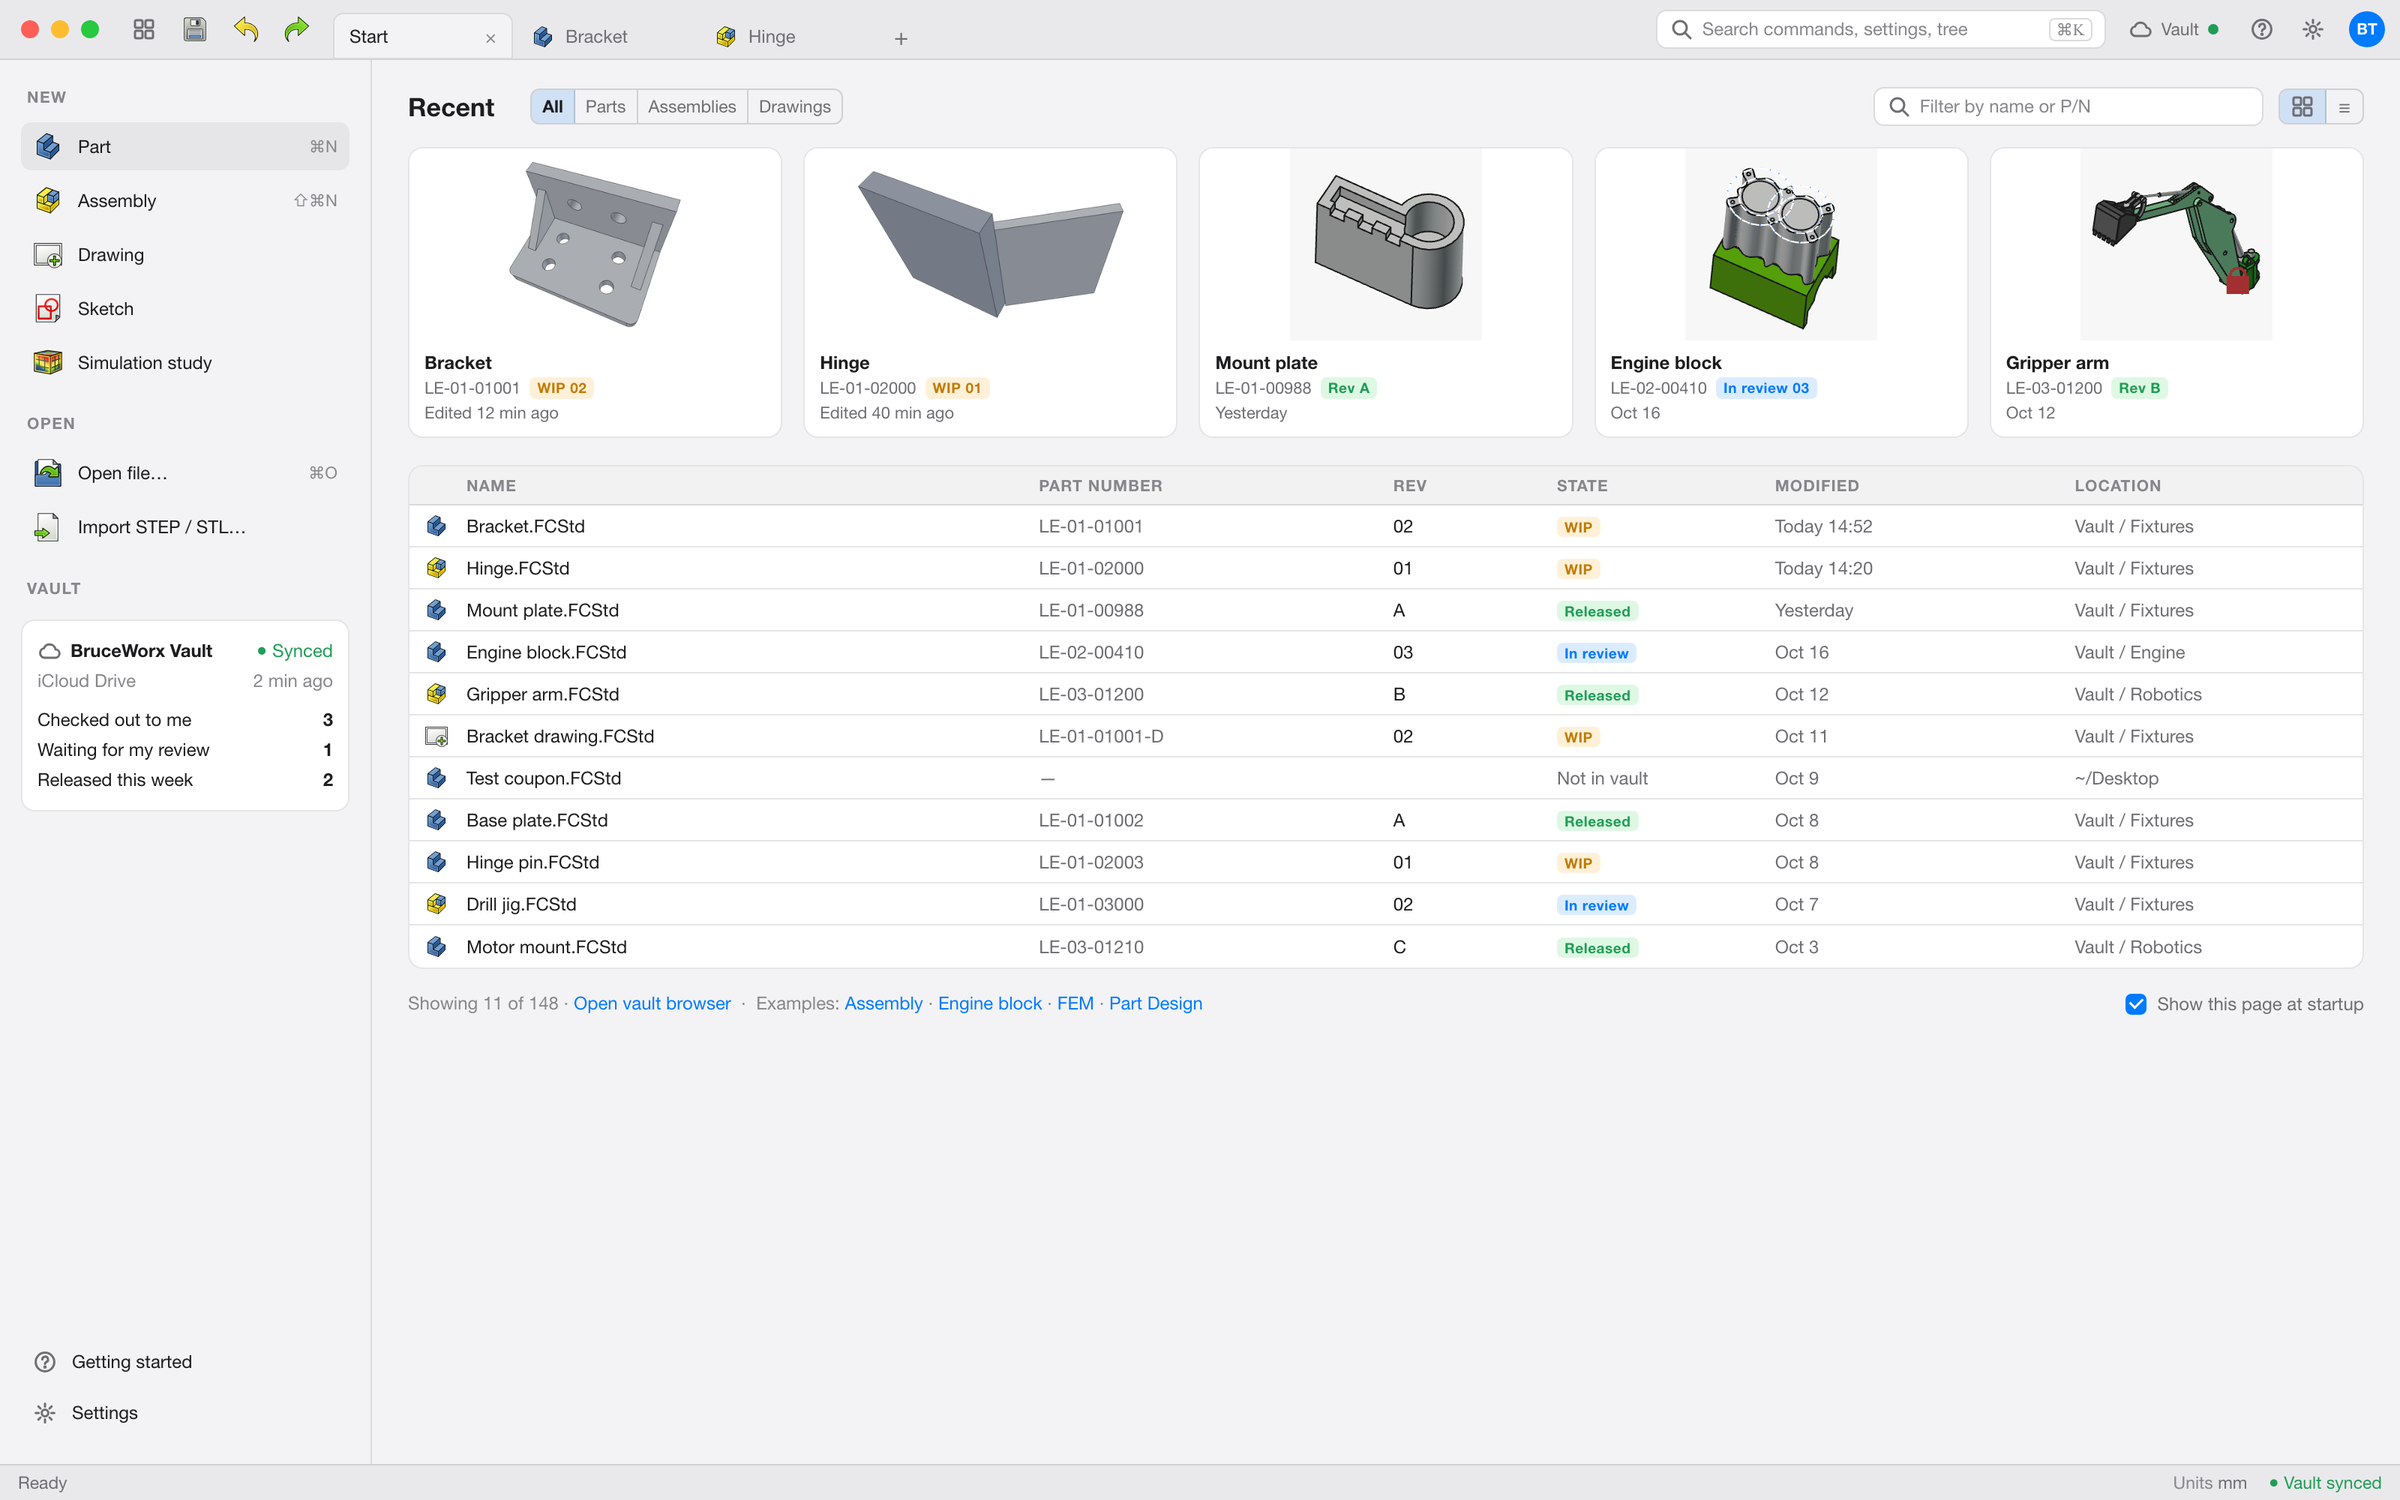
\includegraphics[width=0.497\linewidth]{fig/ui_mock_start-light.png}\hfill
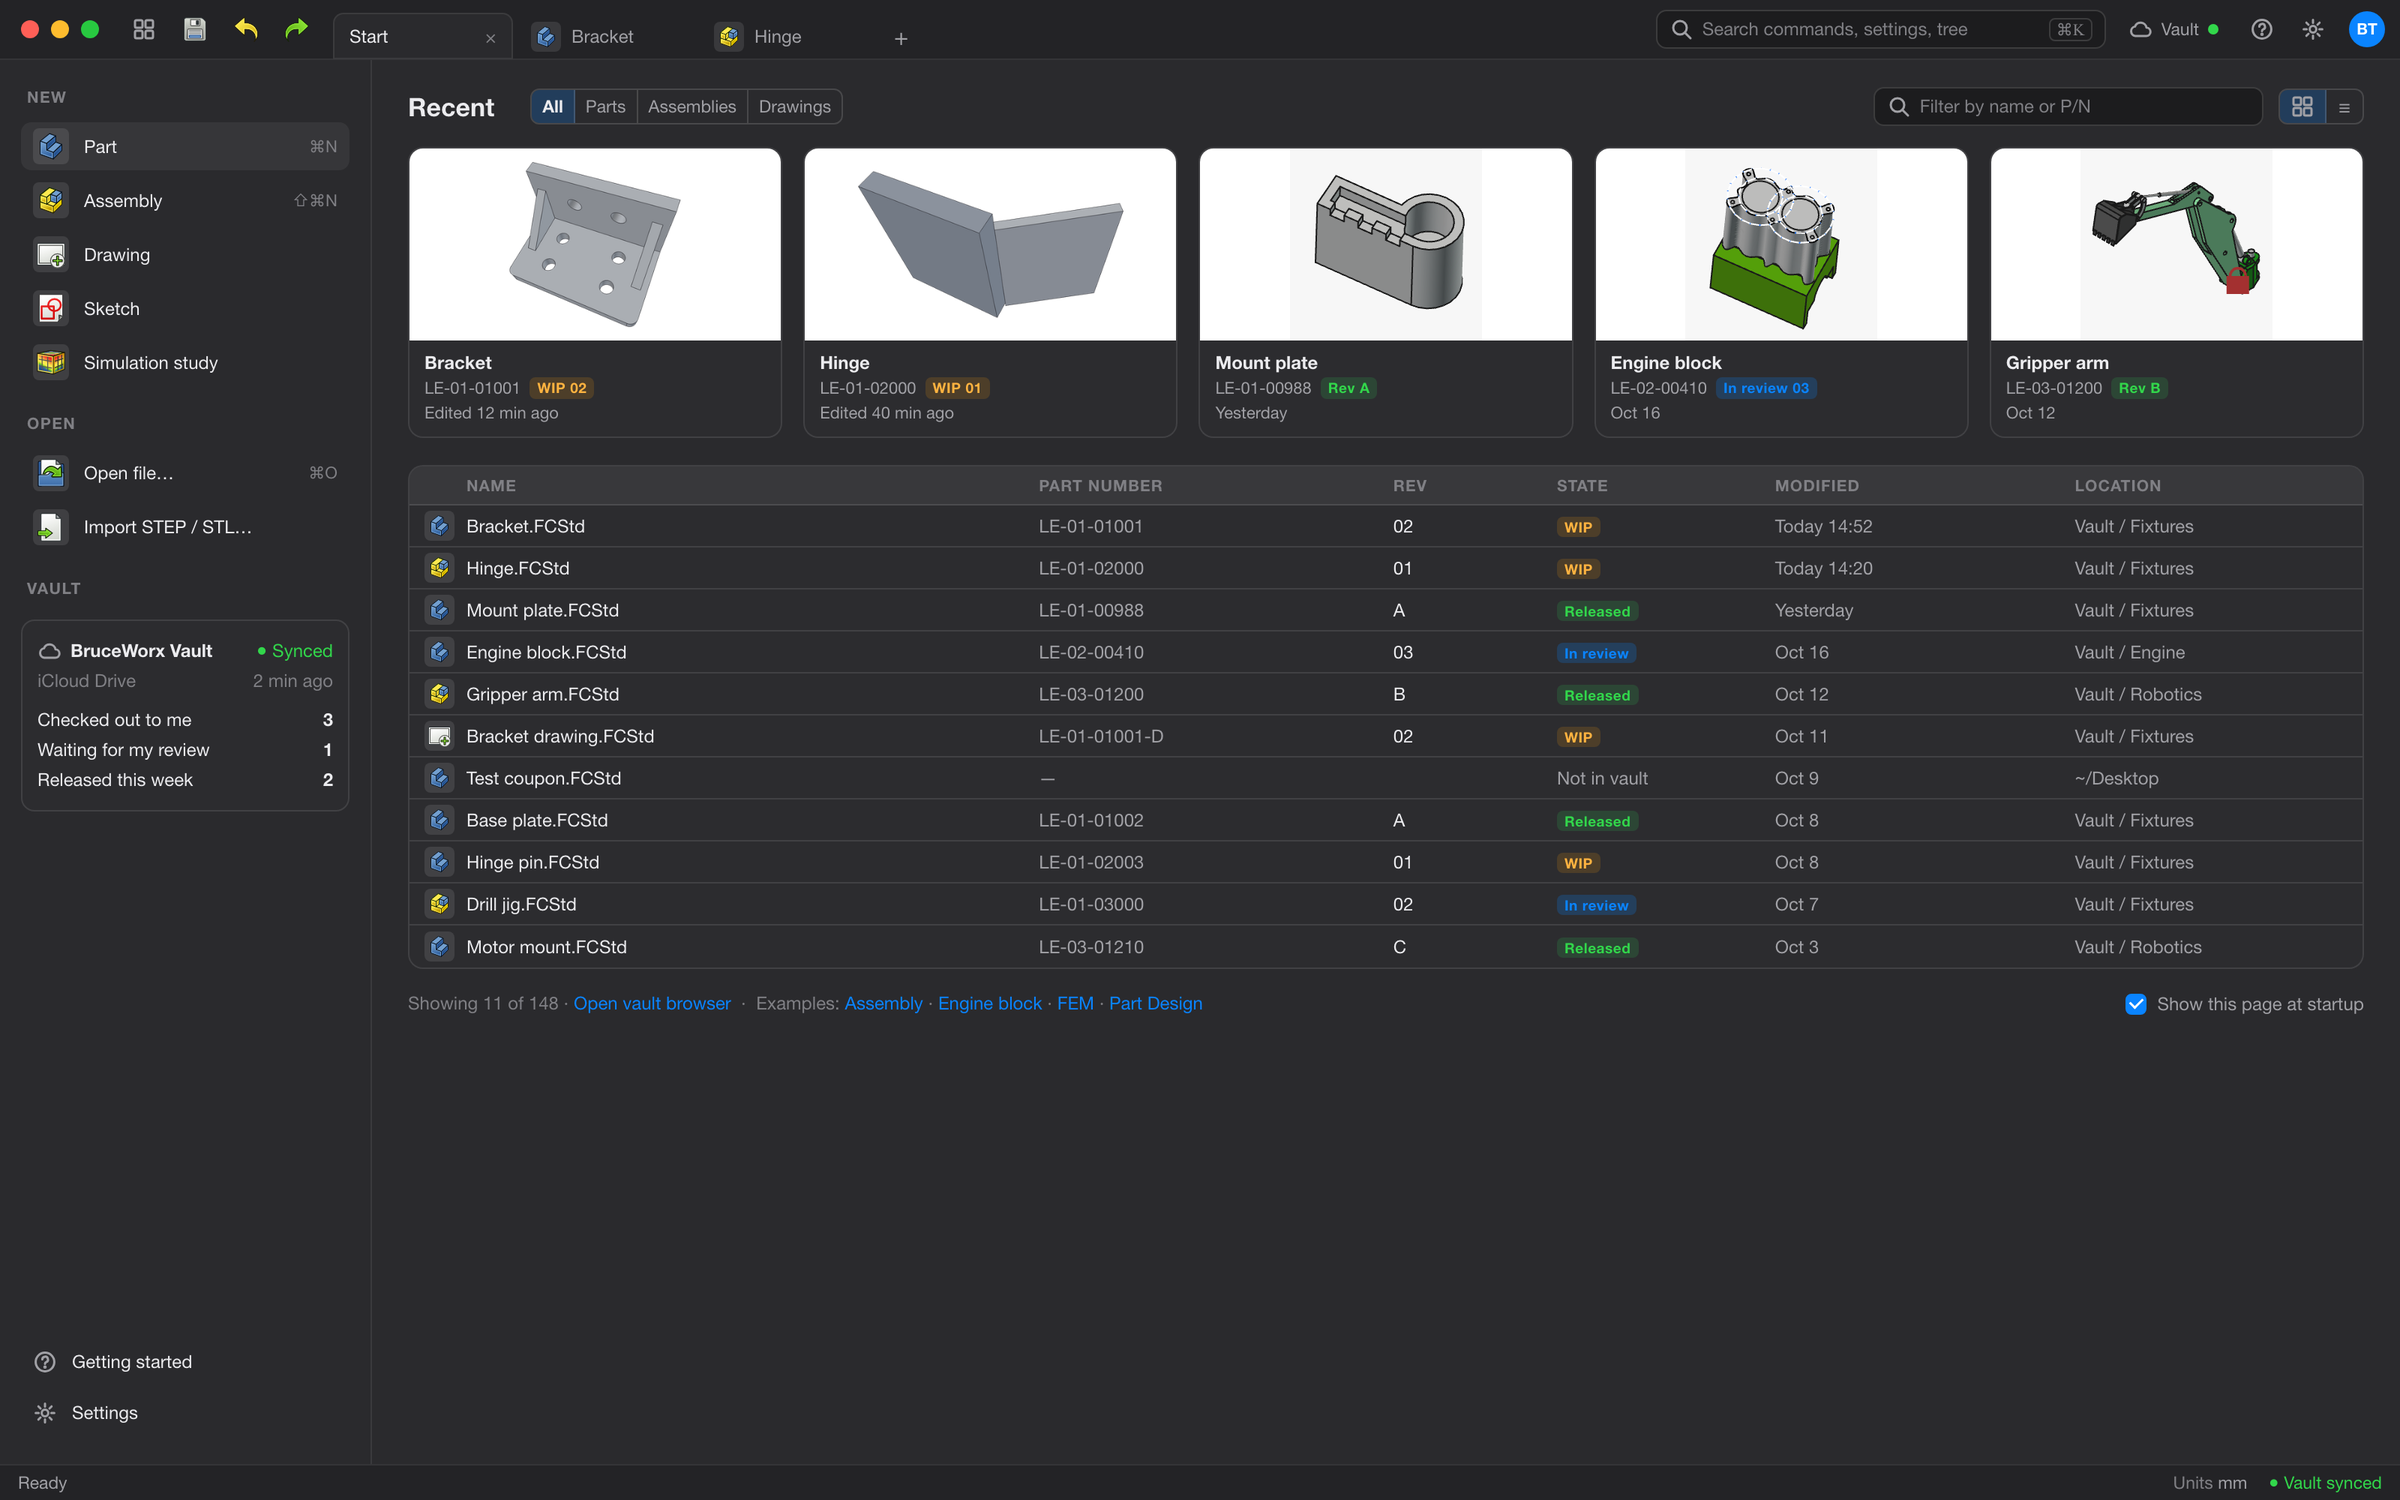
\includegraphics[width=0.497\linewidth]{fig/ui_mock_start-dark.png}
\caption{Sketch and Start page, light and dark.
\emph{Sketch:} the contextual \textsc{Sketch} tab replaces the solid tools, with \textsc{Finish Sketch} at the end. The sketch palette shows the solver (``2 degrees of freedom'', with the free geometry in blue) and a dense constraint list. The timeline is rolled back to the sketch.
\emph{Start:} new and open on the left, with the vault summary; recent files as cards, then as a table with P/N, revision and state.}
\label{fig:ui-sketch-start}
\end{figure}

\paragraph{How following the system works.} FreeCAD 1.1 has no setting for this. It applies one theme
(\file{BruceWorx.yaml} or \file{BruceWorx Dark.yaml}) and one stylesheet at start-up. This build's Qt is 6.8.3,
and Qt reports the system appearance as \code{QStyleHints::colorScheme()}, with a \code{colorSchemeChanged} signal
when you switch. BruceWorx listens for that signal. It loads the matching yaml colour tokens, re-applies
\file{BruceWorx.qss} (already written once for both themes), and sets the two viewport background colours and the
NaviCube colours. No restart is needed. The accent comes from \code{QPalette::Accent} (Qt~6.6 and later), which
on macOS is the System Settings accent. It is written into the \code{@AccentColor} token, and the derived tokens
are computed from it:
\[
  \text{accent-soft} = \alpha\,A + (1-\alpha)\,B, \qquad \alpha = 0.14 \text{ (light)},\ 0.22 \text{ (dark)},
\]
where $A$ is the accent and $B$ the card colour. Selected rows, pressed tools and chips use accent-soft. Only the
default button, checkboxes and the focus ring use the full accent.

\paragraph{Contrast, checked rather than eyeballed.} With a user-chosen accent, text on it can become
unreadable (white on yellow). The rule uses the WCAG relative luminance of each colour,
\[
  L = 0.2126\,R + 0.7152\,G + 0.0722\,B, \qquad c = \begin{cases} c_s/12.92 & c_s \le 0.04045\\ \left(\tfrac{c_s+0.055}{1.055}\right)^{2.4} & \text{otherwise}\end{cases}
\]
for each sRGB channel $c_s \in [0,1]$, and the contrast ratio $C = (L_1+0.05)/(L_2+0.05)$ with $L_1 \ge L_2$.
Text on the accent is white when $C_\text{white} \ge 3$ (macOS's own choice for buttons), otherwise near-black.

\begin{center}
\small
\begin{tabular}{@{}lrr@{\qquad}lrrl@{}}
\toprule
Text on card & Light & Dark & macOS accent & White & Black & Text\\
\midrule
Primary & 16.8 & 11.8 & Blue & 4.02 & 5.23 & white\\
Secondary & 5.1 & 5.4 & Purple & 4.88 & 4.31 & white\\
Tertiary (hints) & 3.6 & 3.5 & Pink / Red & 3.20 / 3.18 & 6.6 & white\\
\textit{Faded tree today} & \textit{1.1} & --- & Orange & 2.57 & 8.16 & black\\
 & & & Yellow / Green & 1.58 / 2.43 & 13.3 / 8.6 & black\\
\bottomrule
\end{tabular}
\end{center}
The mock's tertiary grey was darkened from 2.6:1 to 3.6:1 by this check. The accent values are Apple's published
light-mode colours. \verify

\begin{center}
\small
\begin{tabular}{@{}lll@{\qquad}lll@{}}
\toprule
Token & Light & Dark & Token & Light & Dark\\
\midrule
Chrome & \code{\#E9E9EC} & \code{\#232326} & Text & \code{\#1D1D1F} & \code{\#ECECEF}\\
Toolbar & \code{\#F3F3F5} & \code{\#2A2A2D} & Text 2 & \code{\#6E6E73} & \code{\#A1A1A6}\\
Card & white 88\,\% & \code{\#262629} 90\,\% & Text 3 & \code{\#86868B} & \code{\#808085}\\
Field & \code{\#FFFFFF} & \code{\#1C1C1E} & Accent & system & system\\
Viewport top & \code{\#FBFBFC} & \code{\#4A4F57} & OK & \code{\#1F9D55} & \code{\#32D74B}\\
Viewport bottom & \code{\#DFE3E9} & \code{\#26292E} & WIP & \code{\#C27C00} & \code{\#FFB340}\\
\bottomrule
\end{tabular}
\end{center}

\subsubsection*{Before and after}

\begin{figure}[!htbp]
\centering
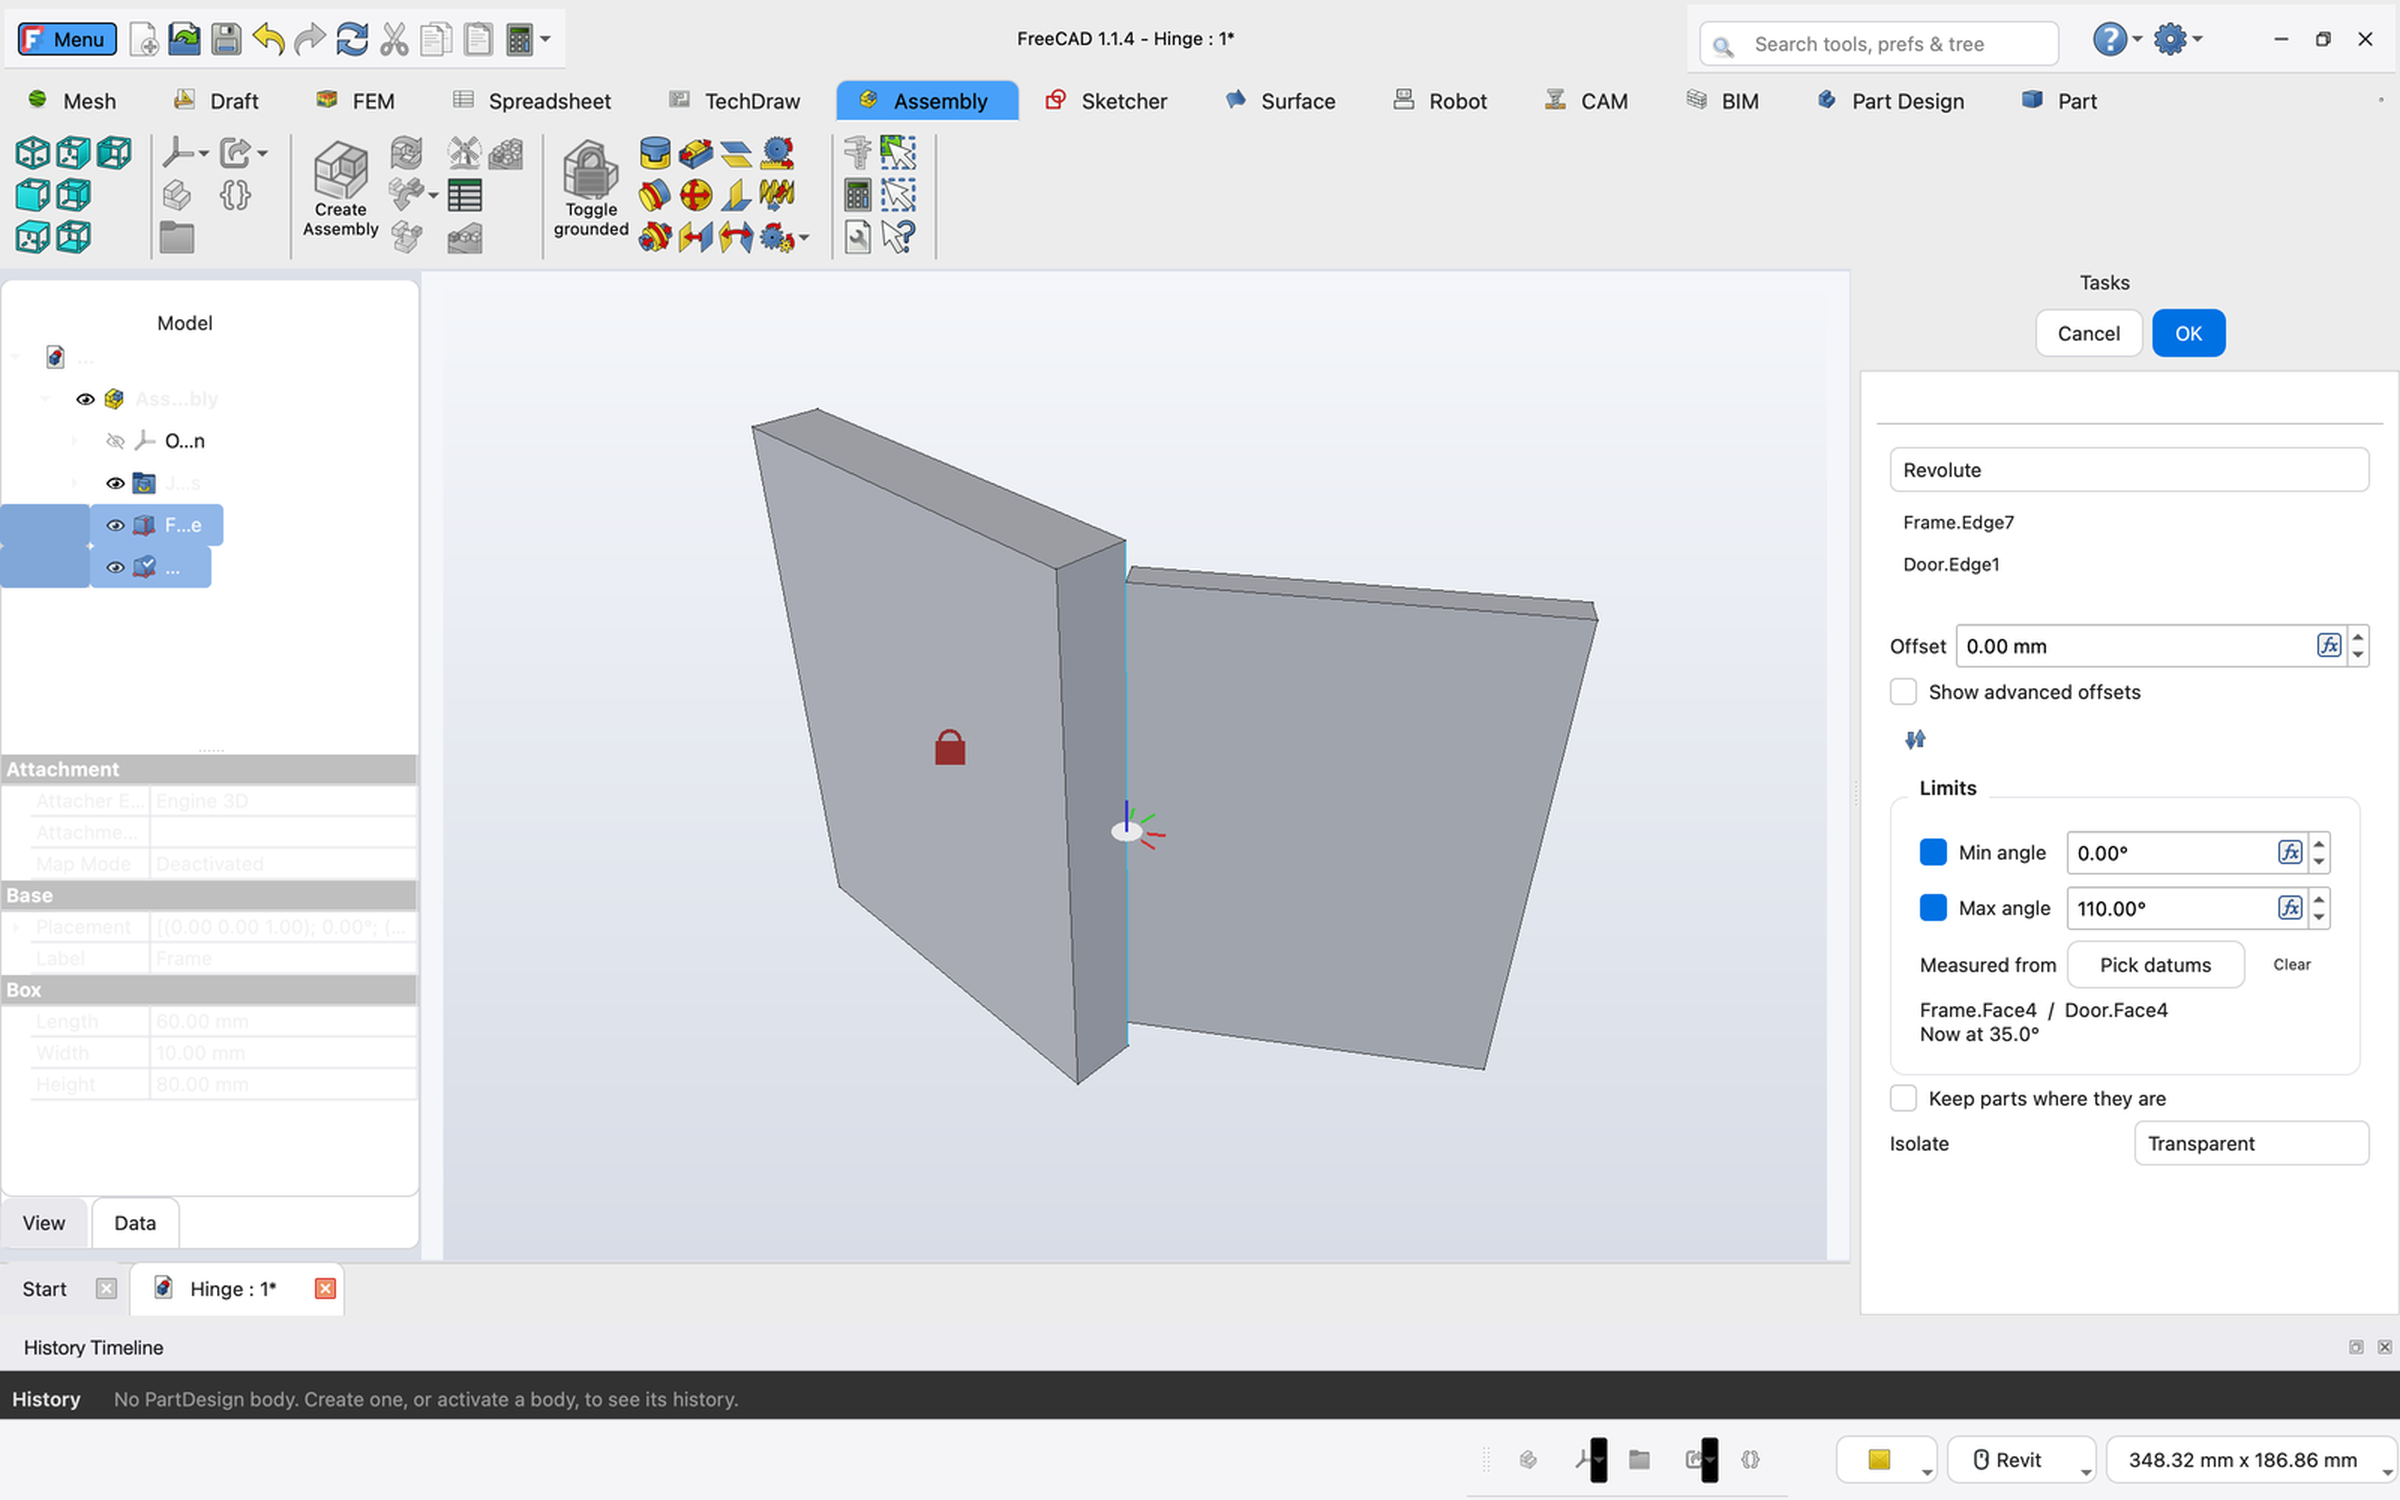
\includegraphics[width=0.497\linewidth]{fig/ui_before_joint.png}\hfill
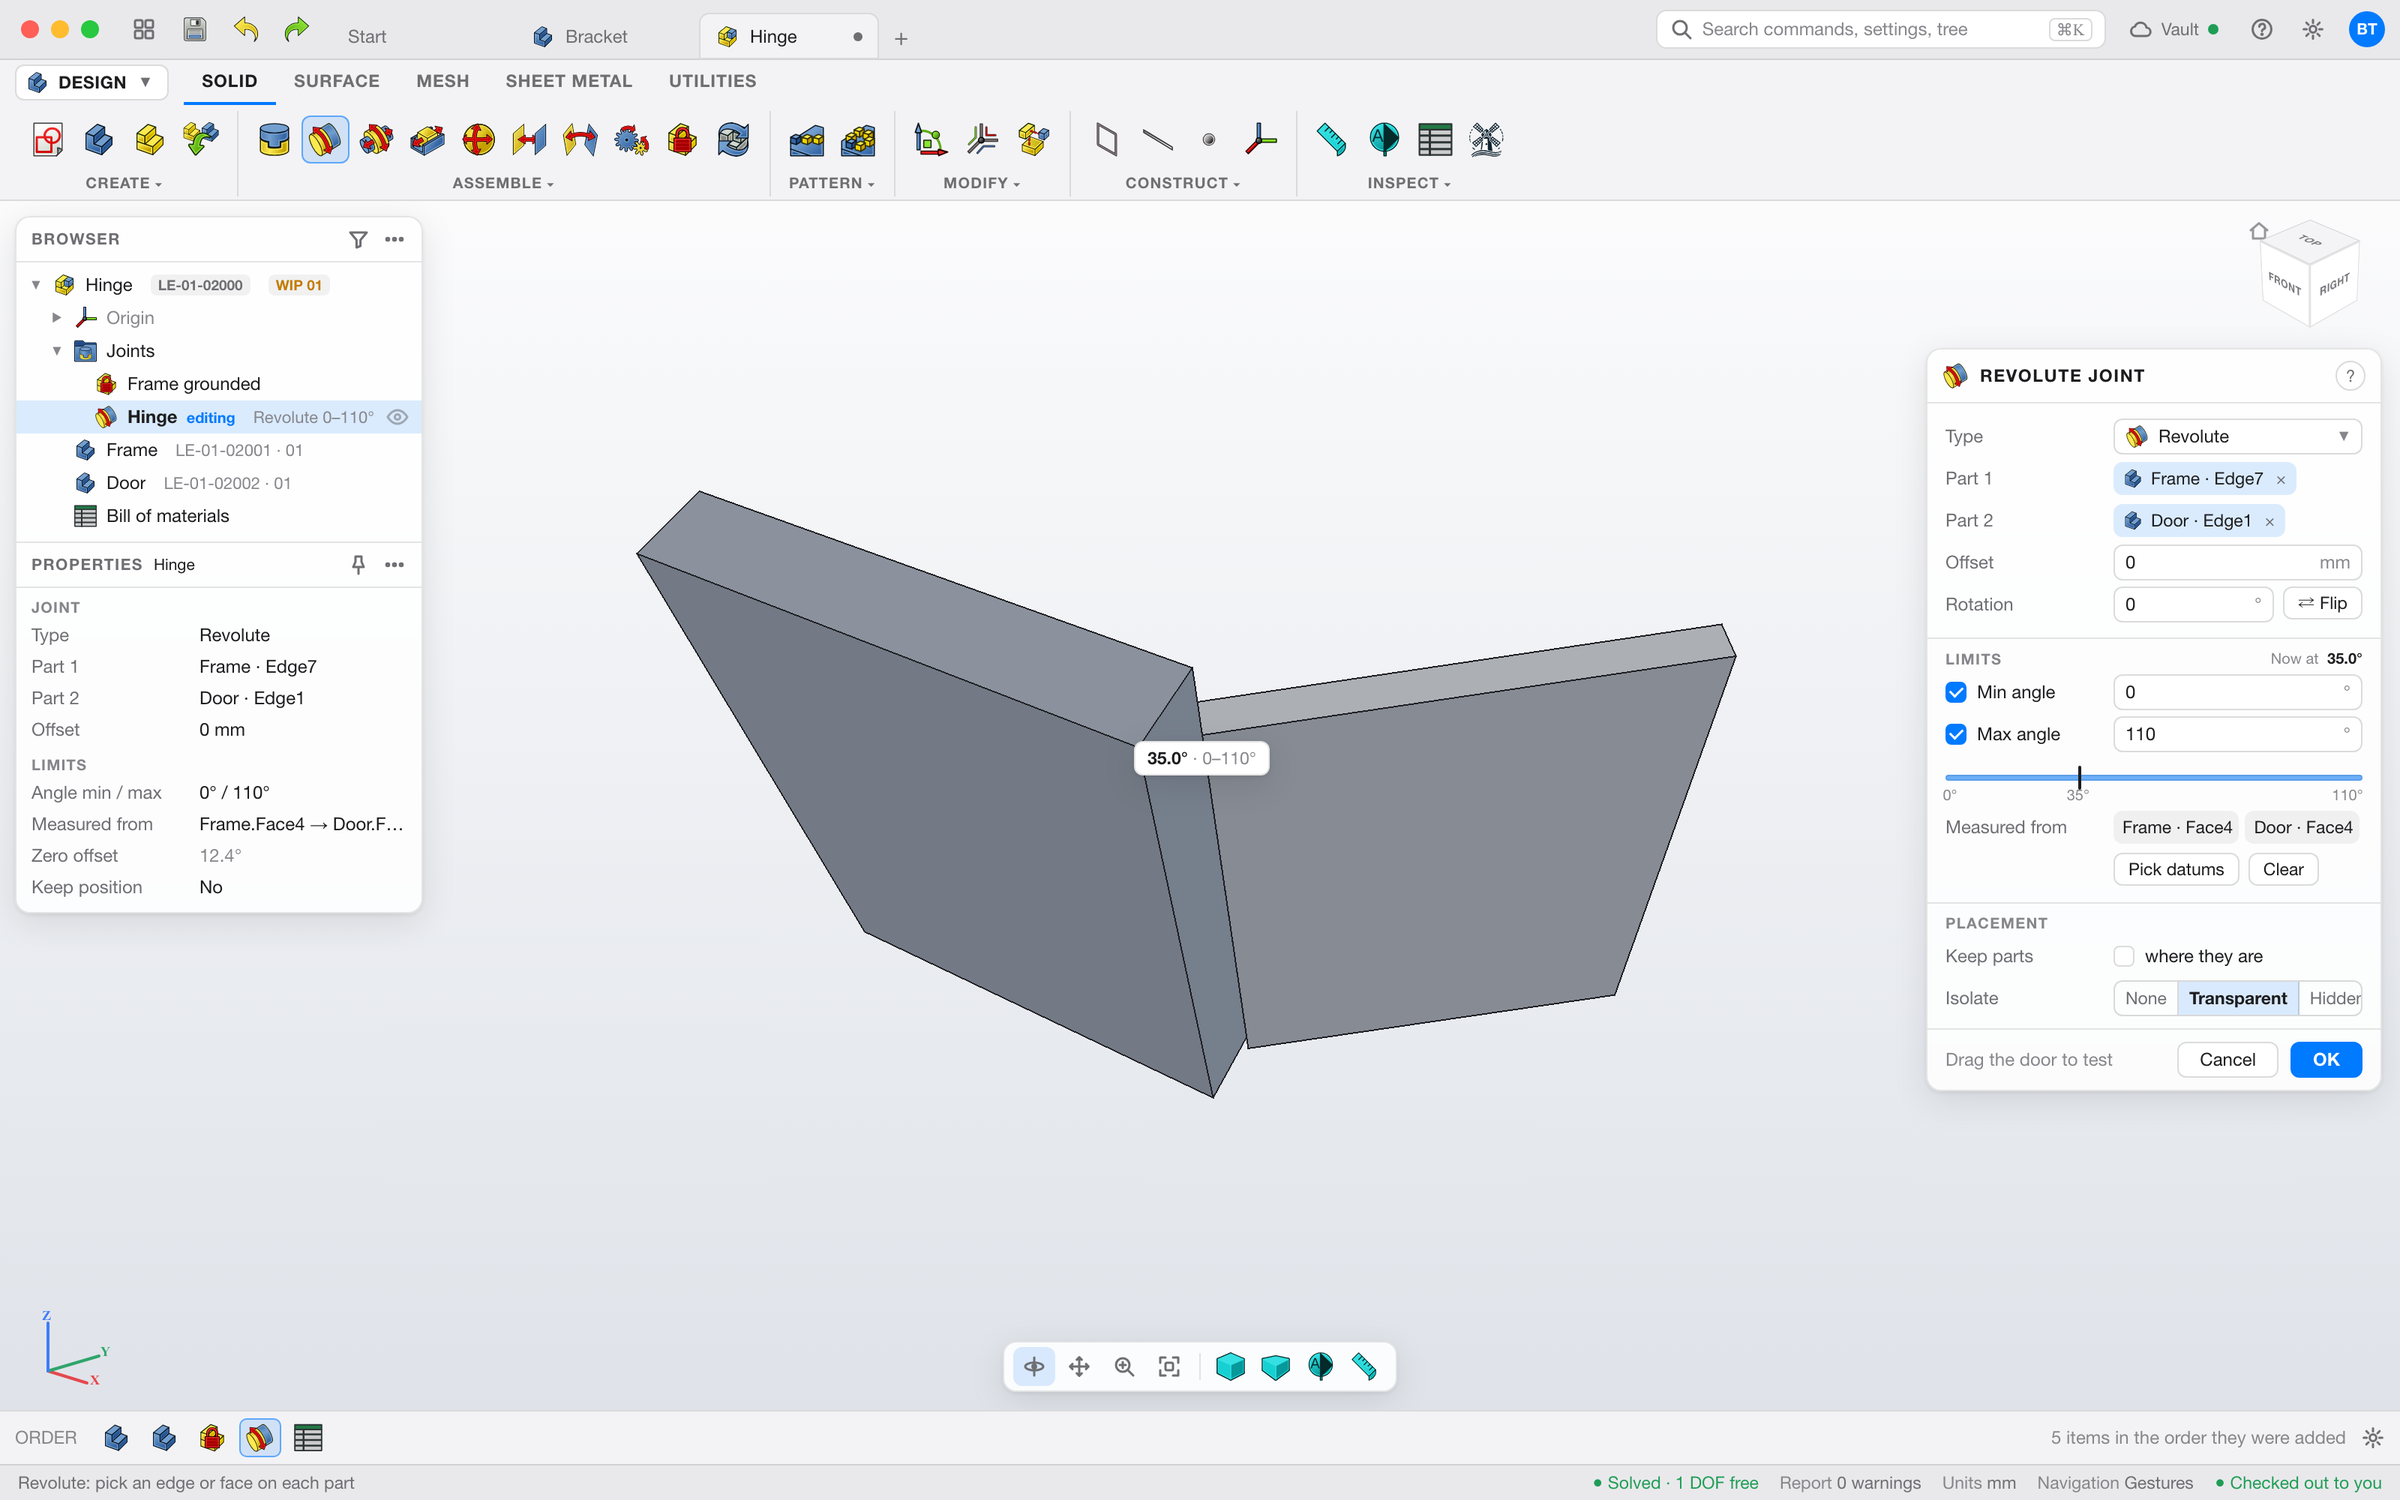
\includegraphics[width=0.497\linewidth]{fig/ui_mock_asm-light.png}
\caption{The same joint, today (left) and in the mock (right).}
\label{fig:ui-before-after}
\end{figure}

\subsubsection*{Plan: three steps, each shown before and after}

Each step ends with the four screens captured from the real build in light and dark, next to these mocks, for you
to approve.

\begin{center}
\small
\begin{tabularx}{\linewidth}{@{}lXl@{}}
\toprule
Step & Work & Size\\
\midrule
\textbf{A. Stylesheet and settings} & Colour tokens and sizes above in \file{BruceWorx.qss} and the two yaml files.
  Cards for Browser and dialog. NaviCube settings. Fix \marker{2}\marker{4}\marker{5}\marker{7}\marker{8}\marker{9}\marker{10}
  of figure~\ref{fig:ui-before}. Ribbon off in the BruceWorx profile. No C++.
  & small\\
\textbf{B. Small code} & Follow appearance and accent (signal + token reload). Document tabs on top. Dialog
  buttons at the bottom. Navigation pill. One-row timeline, hidden without history. Status-bar readouts.
  & medium\\
\textbf{C. Structure} & Workspace menu and tabs (\eref{UIX-05}), captioned groups (\eref{UIX-06}), tabs in the
  title bar, search, Start page, Browser badges. & large\\
\bottomrule
\end{tabularx}
\end{center}

\paragraph{Your answers (19 Oct, second round).}
\begin{enumerate}[nosep]
  \item \textbf{Dark-mode icons:} a faint light plate behind each icon in dark mode only, shown first
        (figure~\ref{fig:ui-plates}). The dark figures above already use it at 10\,\%.
  \item \textbf{Search:} ``yes''. Read as the built-in \texttt{Cmd-K} field; to be confirmed.
  \item \textbf{Ribbon add-on:} my call. BruceWorx turns FreeCAD-Ribbon off in its own profile while the
        BruceWorx bar is on and leaves it installed, so turning the bar off brings Ribbon back.
  \item \textbf{Properties:} stay in the Browser card, which grows down to fit them.
  \item \textbf{Assembly timeline:} components and joints in the order they were added. FreeCAD numbers every
        object as it is created (\code{obj.ID}), so the order needs no new data. No playback buttons:
        an assembly has nothing to roll back.
  \item \textbf{Document tabs:} a thin row under the title bar is acceptable if the title bar is impractical.
\end{enumerate}

\begin{figure}[!htbp]
\centering
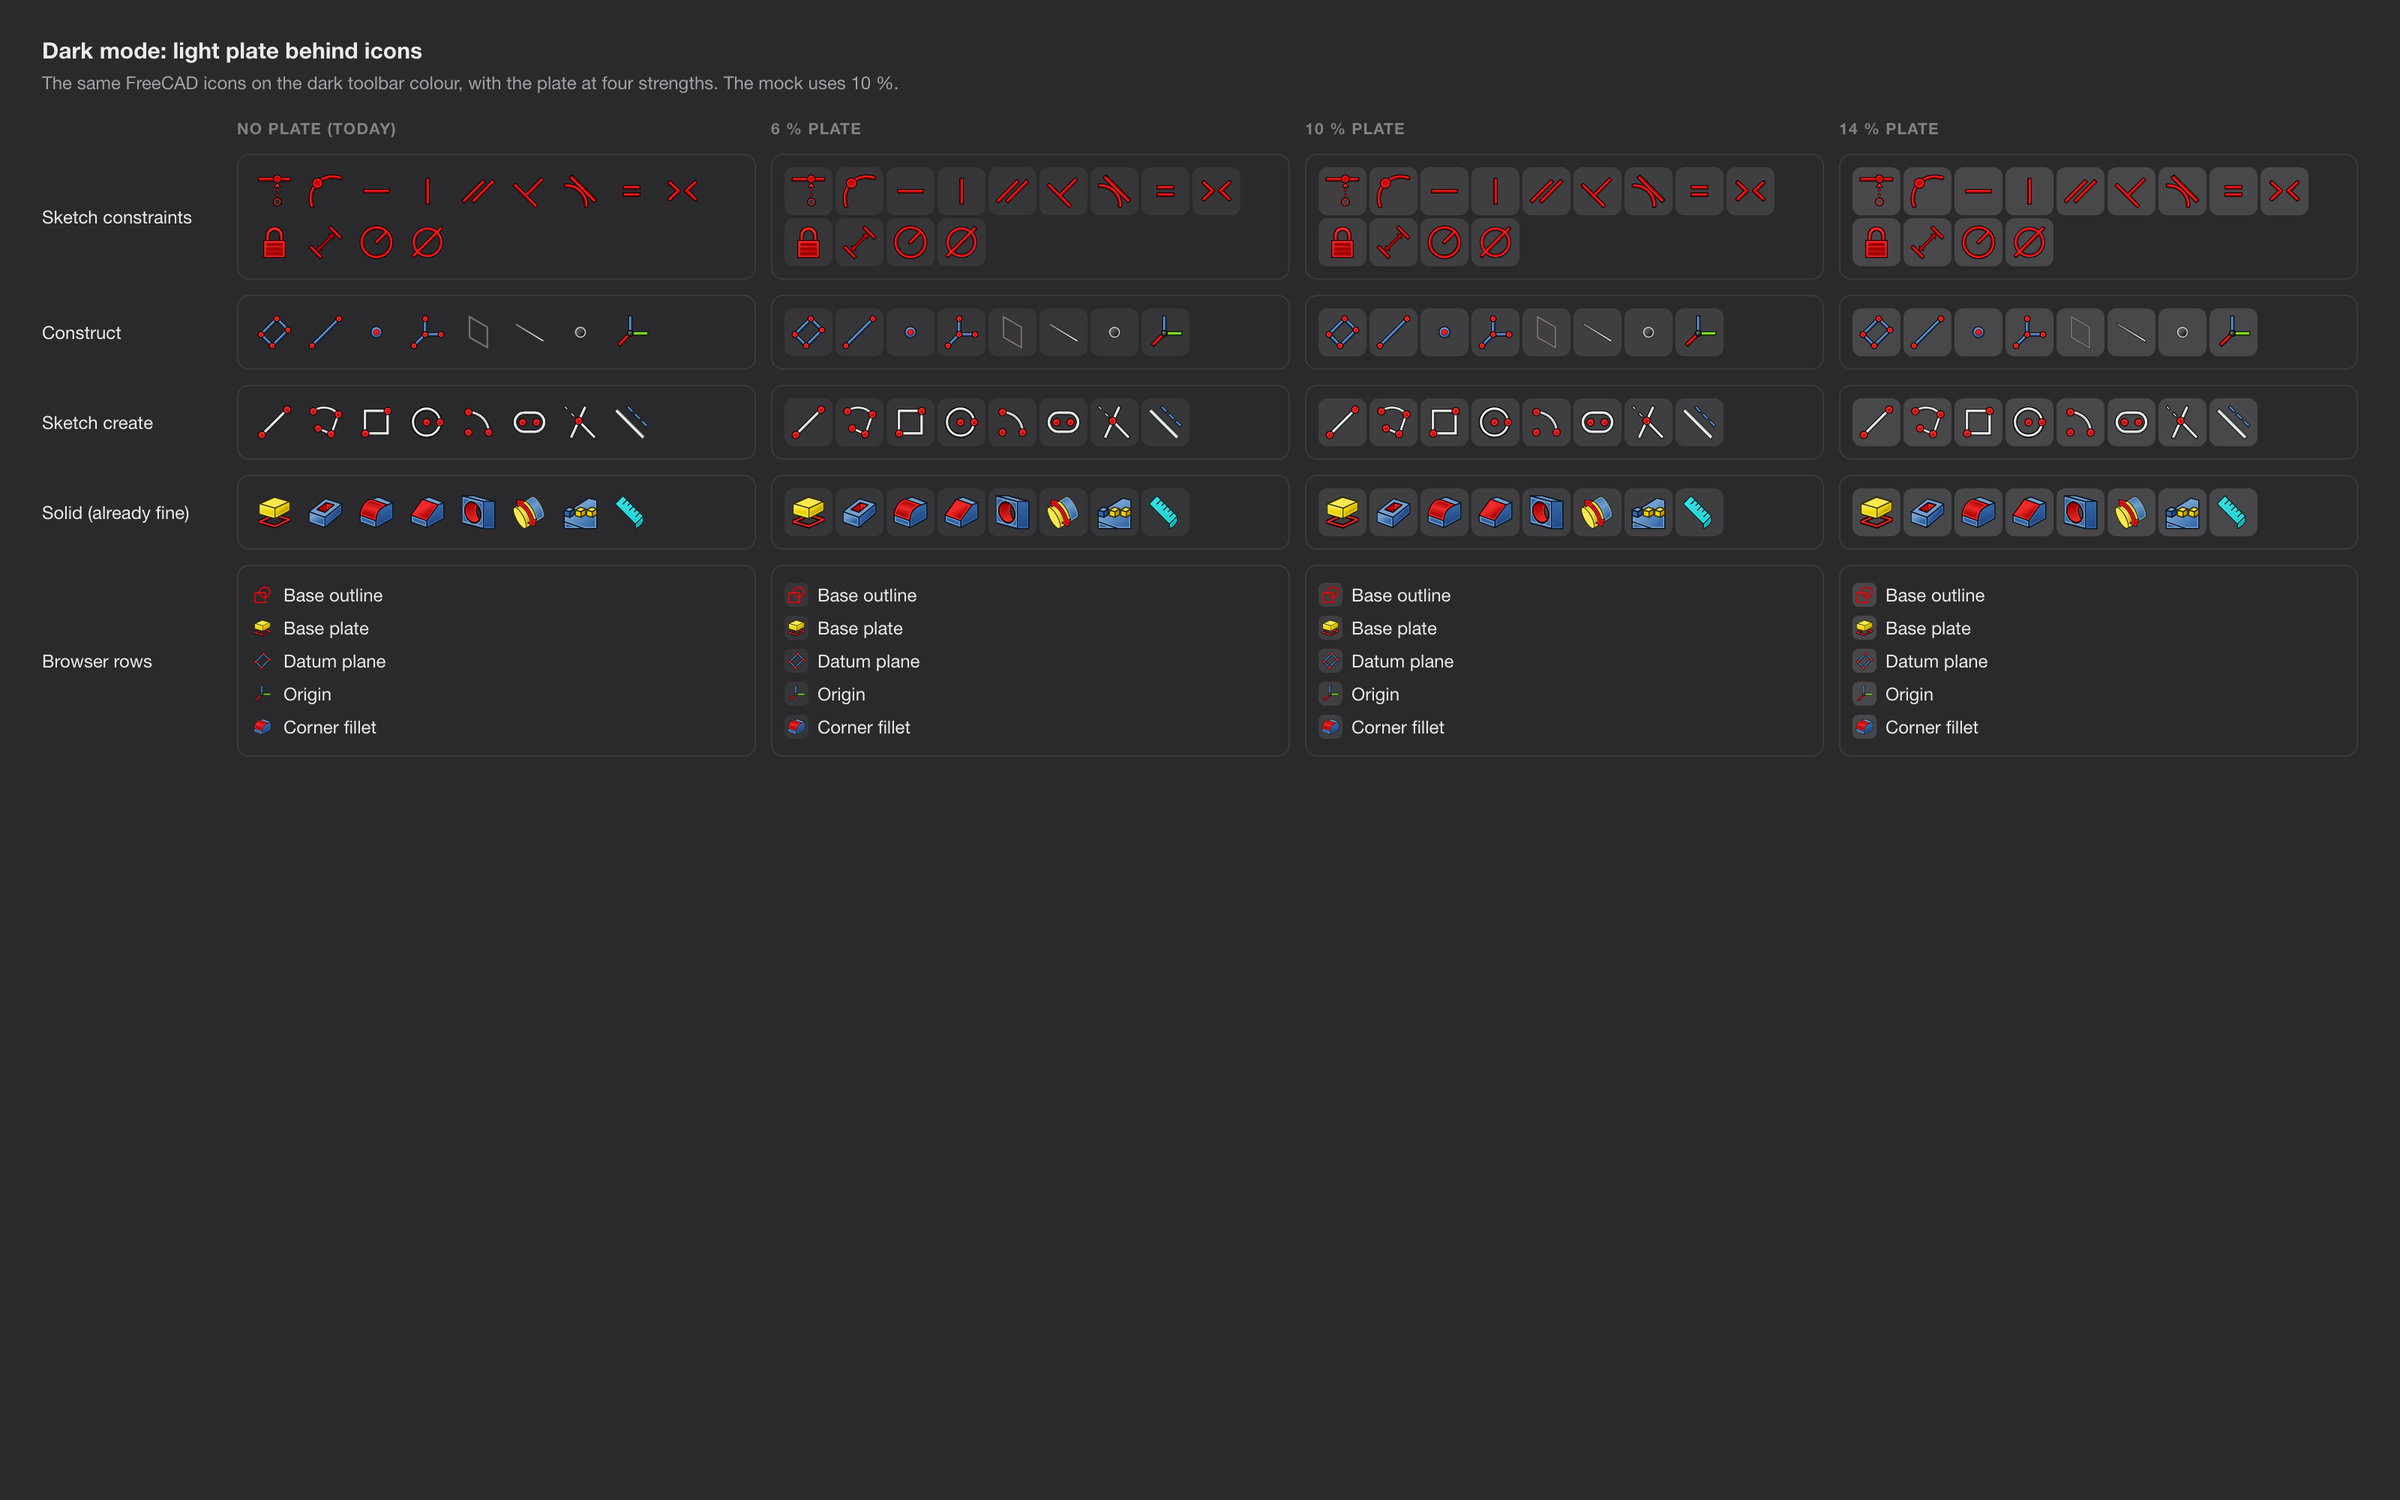
\includegraphics[width=\linewidth]{fig/ui_mock_plates.png}
\caption{Dark mode, the same FreeCAD icons with no plate and with 6, 10 and 14\,\% white plates. The plate lifts
the black-outlined icons (construct, sketch create) clearly. It does much less for the red constraint icons,
whose problem is red on dark rather than outline on dark. In Qt the toolbar plate is one stylesheet rule on the
tool buttons. The plate behind tree and list icons needs a small item delegate (step~B).}
\label{fig:ui-plates}
\end{figure}

\subsubsection*{Step A: done (19 Oct 2026)}

\begin{figure}[!htbp]
\centering
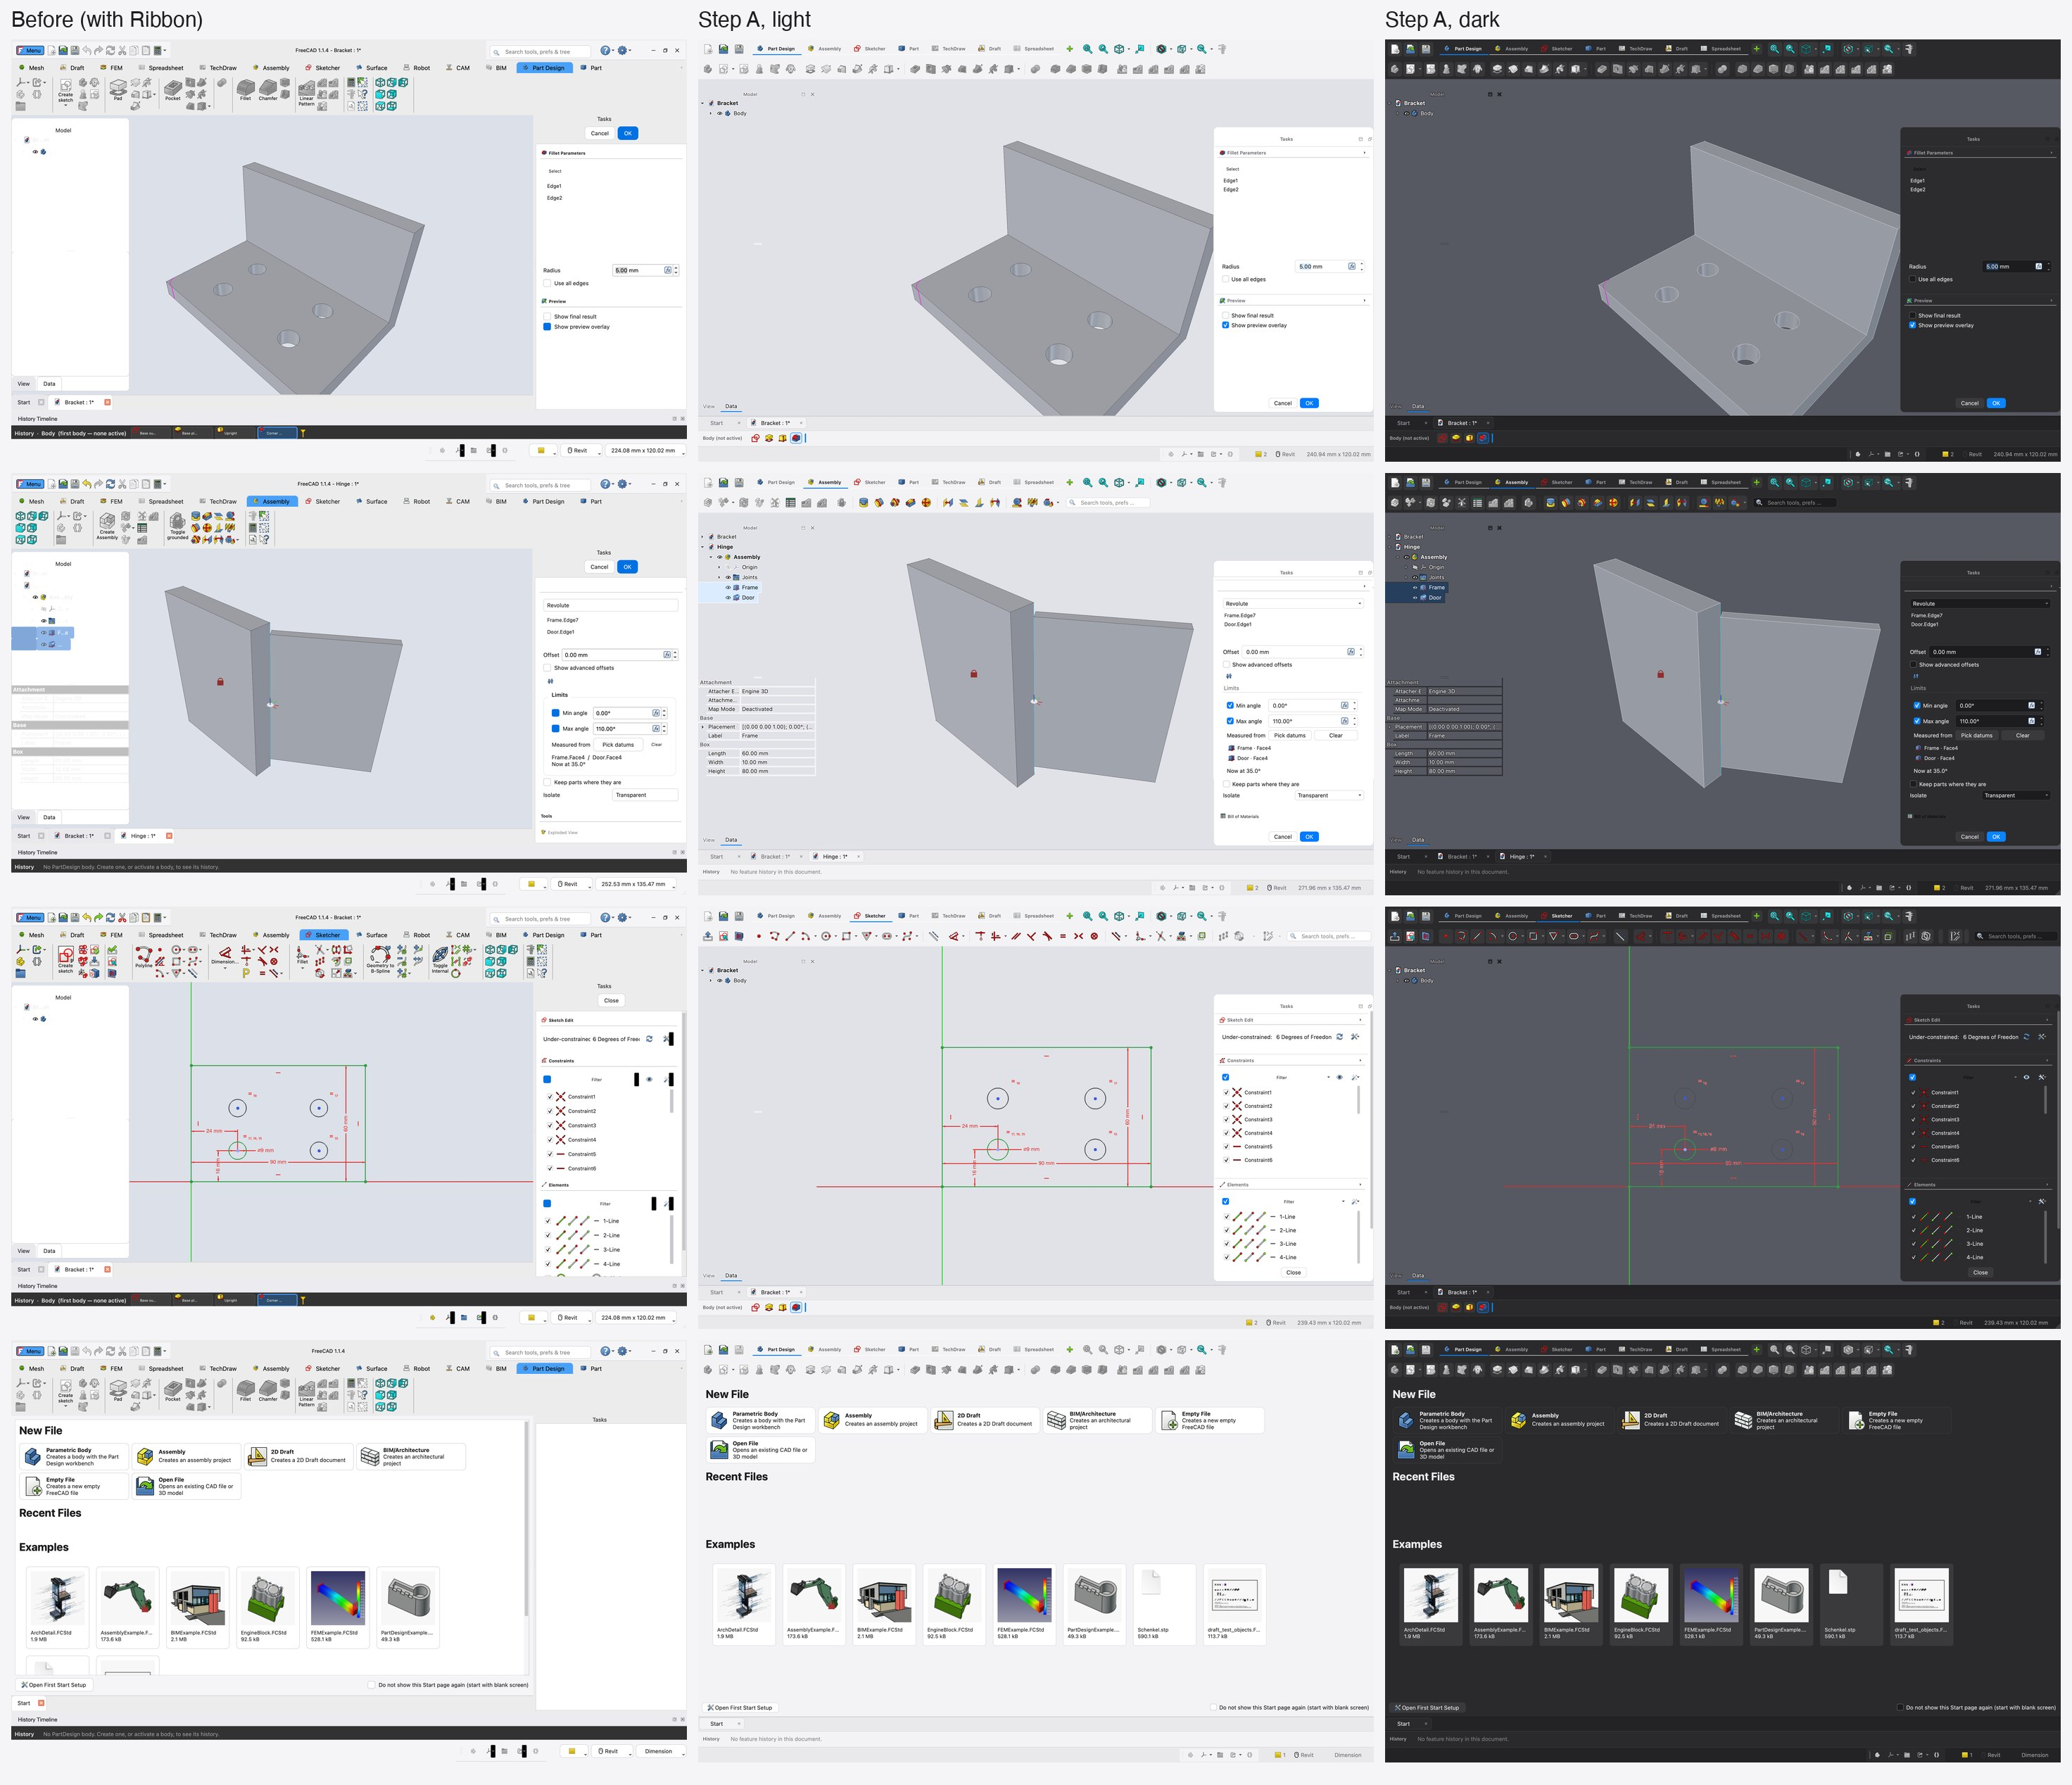
\includegraphics[width=\linewidth]{fig/ui_stepA_sheet.jpg}
\caption{The real build, captured on a copy of your settings: before (Ribbon on), and after step A in light
and dark. Rows: part with a fillet open, the hinge joint, a sketch, the Start page. The 3D view is rendered
separately and pasted in, because a window grab leaves it blank; the view cube is not in these pictures.}
\label{fig:ui-stepA}
\end{figure}

\begin{center}
\small
\begin{tabularx}{\linewidth}{@{}X>{\raggedright\arraybackslash}p{5.1cm}@{}}
\toprule
Change & Where\\
\midrule
Colour tokens from the mock, light and dark; \code{blend()} gives the soft accent & \file{parameters/BruceWorx*.yaml}\\
12\,px type, 22\,px rows, 6/10\,px corners, flat task boxes as cards, thin tab $\times$ & \file{BruceWorx.qss}, \file{close-thin-*.svg}\\
Tree names no longer cut short (horizontal item padding removed) & \file{BruceWorx.qss}\\
Checkboxes show a tick; drop-down tools no longer paint a black bar & \file{BruceWorx.qss}\\
Dark-mode icon plate, 6\,\% white mixed into the toolbar colour (tokens carry no alpha) & \file{BruceWorx Dark.yaml}\\
Browser slightly transparent (your choice): a tinted glass card, 72\,\% opaque, text with a halo & \file{BruceWorx.py}, \file{BruceWorxModelTree.qss}\\
Task panel floats right as one card, shown only while a command is open; its boxes are flat sections & \file{BruceWorx.py}, \file{BruceWorxModelTree.qss}\\
OK/Cancel at the foot of every task panel (dialogs that choose a side keep it) & \file{TaskDialog.cpp}\\
Picks shown as lists: limit datums (Delete removes one), pattern objects & \file{JointObject.py}, \file{bruceworx\_pattern\_gui.py}\\
FreeCAD-Ribbon not loaded while \emph{BruceWorx top bar} is on (stays installed; stock FreeCAD still loads it) & \file{FreeCADInit.py}, \file{FreeCADGuiInit.py}\\
Two toolbar rows after every workbench switch (stale line breaks gave three or four) & \file{bruceworx\_toolbars.py}\\
Timeline: one row of icon chips in theme colours, no dock title, quiet empty message & HistoryTimeline mod\\
Start page readable in dark & \file{BruceWorx.qss}\\
Viewport gradient, accent, selection and view-cube colours from the mock & \file{bruceworx\_pack.py} (cfg regenerated)\\
Sketch grid on, as in the mock (your pick): faint translucent lines (white on dark, black on light), a major line every 5 squares, follows the zoom. The grid now honours a colour's alpha & \file{bruceworx\_pack.py}, \file{ViewProvider\-Grid\-Extension.cpp}\\
\emph{Sketch grid strength} preference, 2--40\,\%, default 10; open sketches update at once. Python: \code{bruceworx\_grid.set\_strength(14)}; a \code{GRID 14} alias comes with the command line (\eref{AUT-05}) & \file{bruceworx\_grid.py}\\
Joint panel \emph{Clear} is a normal button & \file{TaskAssemblyCreateJoint.ui}\\
\bottomrule
\end{tabularx}
\end{center}

New switches on Preferences $\rightarrow$ BruceWorx, all on by default: \emph{BruceWorx top bar}, \emph{Two
toolbar rows}, \emph{Float the task panel}; \emph{Transparent background} is on again by default. OK/Cancel at the
bottom reads \code{BruceWorx/TaskButtonsAtBottom} (no checkbox yet). Tests: 10 BruceWorx, 19 pattern, 16 Assembly, 26 pack, all passing.
To see the new colours on your own profile the pack must be applied again (Preferences $\rightarrow$ General
$\rightarrow$ Preference packs $\rightarrow$ BruceWorx), because a pack writes its values once.

\paragraph{Found on the way.} Editing a \file{.ui} panel does not rebuild the module's \file{\_rc.py}: the build
only watches the \file{.qrc}, and Python loads panels from that file. That was the cause of the stale joint
panel earlier today too. Until the CMake rule is fixed, delete \file{build/release/\{src/Mod/X/Gui,Mod/X\}/X\_rc.py}
after changing a panel.

\paragraph{Left for step B.} Task card header with the command's icon and title (a box without a title still
shows an empty strip); an inset from the right window edge (the overlay pins panels to the edge);
\textsc{Browser} header and badges; navigation pill; timeline in creation order for assemblies and hidden when
there is no history; follow the macOS appearance and accent live; sketch colours (free geometry blue,
constrained in text colour, dimensions quiet); document tabs on top; the property group captions.

\subsubsection*{Step B, in progress}

\paragraph{1. Follow macOS appearance and accent (done).} \file{bruceworx\_appearance.py} listens for Qt's
\code{colorSchemeChanged} and for palette or activation events (macOS has no accent signal). On a light/dark
change it writes only the pack values that differ between the two modes; FreeCAD reloads the stylesheet when the
Theme parameter changes. The accent is read from \code{AppleAccentColor} and written to
\code{ThemeAccentColor1}, which the yaml files now use as \code{@AccentColor}, and to the 3D selection and
view-cube highlight. Text and ticks on the accent follow the contrast rule above: verified live, a yellow
accent gets dark text and dark ticks, blue gets white. Two switches on Preferences $\rightarrow$ BruceWorx, both on.
Theme tokens from \emph{Themes/UserParameters} take precedence over the yaml, so the computed
\code{AccentTextColor} wins over the yaml default.
